%\documentclass[wcp,gray]{jmlr} % test grayscale version
 %\documentclass[wcp]{jmlr}% former name JMLR W\&CP
\documentclass[pmlr]{jmlr}% new name PMLR (Proceedings of Machine Learning)

\RequirePackage{graphicx}
 % The following packages will be automatically loaded:
 % amsmath, amssymb, natbib, graphicx, url, algorithm2e
 \usepackage{booktabs}
 %\usepackage{rotating}% for sideways figures and tables
\usepackage{longtable}
\usepackage{float}
\usepackage{adjustbox}% for long tables
\usepackage[capitalize,noabbrev]{cleveref}
\usepackage{multicol}
\usepackage{multirow}
 % The booktabs package is used by this sample document
 % (it provides \toprule, \midrule and \bottomrule).
 % 
 % book quality tables

%%%%%%%%%%%%%%%%%%
\usepackage{listings}
\usepackage{xcolor}

\definecolor{codegreen}{rgb}{0,0.6,0}
\definecolor{codegray}{rgb}{0.5,0.5,0.5}
\definecolor{codepurple}{rgb}{0.58,0,0.82}
\definecolor{backcolour}{rgb}{0.95,0.95,0.92}

\lstdefinestyle{mystyle}{
    backgroundcolor=\color{backcolour},   
    commentstyle=\color{codegreen},
    keywordstyle=\color{magenta},
    numberstyle=\tiny\color{codegray},
    stringstyle=\color{codepurple},
    basicstyle=\ttfamily\footnotesize,
    breakatwhitespace=false,         
    breaklines=true,                 
    captionpos=b,                    
    keepspaces=true,                 
    numbers=left,                    
    numbersep=5pt,                  
    showspaces=false,                
    showstringspaces=false,
    showtabs=false,                  
    tabsize=2
}

\lstset{style=mystyle}
%%%%%%%%%%%%%%%%%%
 

 % The siunitx package is used by this sample document
 % to align numbers in a column by their decimal point.
 % Remove the next line if you don't require it.
\makeatletter
\def\set@curr@file#1{\def\@curr@file{#1}} %temp workaround for 2019 latex release
\makeatother
\usepackage[load-configurations=version-1]{siunitx} % newer version

 % The following command is just for this sample document:
\newcommand{\cs}[1]{\texttt{\char`\\#1}}

 % Define an unnumbered theorem just for this sample document:
\theorembodyfont{\upshape}
\theoremheaderfont{\scshape}
\theorempostheader{:}
\theoremsep{\newline}
\newtheorem*{note}{Note}

 % change the arguments, as appropriate, in the following:
\jmlrvolume{[VOLUME \# TBD]}
\jmlryear{2024}
\jmlrworkshop{Machine Learning for Healthcare}

% H: Not sure if we need this:
% Short headings should be running head and authors last names
% \ShortHeadings{A Really Awesome MLHC Article}{Lastname, PhD and Lastname, MD}
% \firstpageno{1}

\title[Emergency Department Decision Support]{Emergency Department Decision Support using \\Clinical Pseudo-notes}

\author{\Name{Simon A. Lee}
       \Email{simonlee711@g.ucla.edu}\\ 
       \addr Department of Computational Medicine\\
       University of California, Los Angeles\\
       Los Angeles, California, USA 90095 
       \AND
       \Name{Sujay Jain}
       \Email{jainsujay@g.ucla.edu}\\ 
       \addr Department of Electrical and Computer Engineering\\
       University of California, Los Angeles
       \AND
       \Name{Alex Chen}
       \Email{ashchen@g.ucla.edu}\\ 
       \addr Department of Computational Medicine\\
       University of California, Los Angeles
       \AND
       \Name{Kyoka Ono$^{1,2}$}
       \Email{kyokaono8800@g.ucla.edu}\\ 
       \addr$^1$ Department of Statistics and Data Science\\
       University of California, Los Angeles, \\ 
       $^2$ Department of Natural Sciences\\
       International Christian University,\\
       Mitaka, Tokyo, Japan
       \AND
       \Name{Akos Rudas}
       \Email{akosrudas@g.ucla.edu}\\ 
       \addr Department of Computational Medicine\\
       University of California, Los Angeles
       \AND
       \Name{Jennifer Fang$^{1,2}$}
       \Email{jfang@dhs.lacounty.gov}\\ 
       \addr $^1$ Department of Emergency Medicine\\
        Harbor-UCLA Medical Center,\\
        $^2$Enterprise Clinical Informatics, \\ LA Health Services, Torrance, CA
       \AND
       \Name{Jeffrey N. Chiang$^{1,2}$}
       \Email{njchiang@g.ucla.edu}\\ 
       \addr $^1$Department of Computational Medicine,\\
       $^2$Department of Neurosurgery \\
       University of California, Los Angeles}

\begin{document}

\maketitle
\vspace*{-1cm}
\begin{abstract}
In this work, we introduce the Multiple Embedding Model for EHR (MEME), an approach that serializes multimodal EHR tabular data into text using \iffalse{our}\fi ``pseudo-notes'', mimicking clinical text generation. \iffalse{method}\fi This conversion \iffalse{from tabular to text}\fi not only preserves better representations of categorical data and learns contexts but also enables the effective employment of pretrained foundation models for rich feature representation. To address potential issues with context length, our framework encodes embeddings for each EHR modality separately. We demonstrate the effectiveness of MEME by applying it to several {decision support} tasks within the Emergency Department across multiple hospital systems. Our findings indicate that MEME outperforms {traditional machine learning, EHR-specific foundation models, and general LLMs} \iffalse{other machine learning} methods\fi {, highlighting its potential as a general and extendible EHR representation strategy.} \iffalse{in EHR, underscoring its effectiveness}\fi
% However, we also observe notable limitations in generalizability across hospital institutions for all tested models.
\end{abstract}

\section{Introduction}
In recent years, increased access to Electronic Health Records (EHR) has provided healthcare systems with valuable insights into patients' health histories \citep{idowu2023streams}. This wealth of information makes EHR indispensable for inference tasks, especially as the machine learning community increasingly focuses on healthcare applications. Both traditional and cutting-edge machine learning techniques have been harnessed to aid in specific diagnosis and prognosis tasks \citep{shickel_deep_2018}, with a recent keen interest in incorporating state-of-the-art foundation models, such as Large Language Models (LLMs) \citep{zhao_survey_2023}. These advanced models, pre-trained on extensive and diverse textual corpora, offer a broad understanding across numerous domains, \iffalse{significantly}\fi enhancing their adaptability and effectiveness for various complex tasks. Notably, their ability to generate high-fidelity latent representations can be directly employed in many classification tasks, often demonstrating state-of-the-art performance. However, the adoption of these models, built for natural language and text, has been hampered by the fact that the canonical form of generally available EHR data is tabular, and access to textual clinical notes is generally infeasible due to privacy concerns.

We are particularly interested in integrating Electronic Health Records with Large Language Models because traditional machine learning paradigms often struggle with the heterogeneous nature of EHR data. EHRs are disparate data sources, encompassing a wide array of data types, including numerical (e.g., lab test results), categorical (e.g., diagnosis codes, medication types), and free-text data, while spanning multiple biological domains and scales. This diversity enables comprehensive insights into patient health, treatments, and outcomes but also presents numerous challenges. For instance, EHRs frequently include categories with a large number of classes. Traditional methods like one-hot encoding and conventional feature engineering can obscure the inherent meanings within this data, leading to issues such as inefficient data ingestion, a lack of contextual understanding, and sparse data representations. Addressing these challenges is crucial for making full use of the rich, yet complex, information EHR systems contain.

Therefore, in this work, we introduce the \textit{Multiple Embedding Model for EHR (MEME)}, an approach that processes tabular health records and generates textual representations via our ``pseudonotes'' method. Using these clinical pseudo-notes, MEME bridges the gap between tabular EHR data and modern Natural Language Processing (NLP) techniques. We also find that adopting a multiple embedding strategy, where different components of the EHR are encoded separately, yields better results compared to trying to fit all our text into a single heterogenous embedding. We demonstrate this utility by benchmarking MEME against other EHR methods on prediction tasks related to the emergency department. This is an important problem in both machine learning and healthcare because utilizing a patients health history can help predict future events or requirements needed from the emergency department with high precision.

% XX is an important problem in machine learning and healthcare.  (Make
% sure that the clinicians can see the relevance! \emph{Unclear clinical
%   relevance is a major reason that otherwise strong-looking papers are
%   scored low/rejected.})

% Addressing this problem is challenging because XX.  (Make sure that
% you connect to the machine learning here.)  

% Others have tried, but XX remains tough.  (Acknowledge related work.)

% In this work, we...

% As you write, keep in mind that MLHC papers are meant to be read by
% computer scientists and clinicians.  In the later sections, you might
% have to use some medical terminology that a computer scientist may not
% be familiar with, and you might have to use some math that a clinician
% might not be familiar with.  That's okay, as long as you've done your
% best to make sure that the core ideas can be understood by an informed
% reader in either community.

\subsection*{Generalizable Insights about Machine Learning in the Context of Healthcare}
% In this work, we detail the advantages of operating in a textual modality compared to the traditional tabular form. We will also justify our methods and models by providing a comprehensive evaluation of model selection and performance against other models found in the literature. Furthermore, we underscore the significance of this methodology in a clinical context, as it has the potential to streamline decision making within overcrowded hospital settings by predicting outcomes in advance.

In this work, we evaluate text serialization as an interface between tabular electronic health records and large language foundation models. We find our multimodal text serialization approach which separately considers EHR components and leverages the general reasoning capacity of language foundation models outperforms existing  models specifically tailored for healthcare, and that task-specific tuning further outperforms prompting-based approaches. While we demonstrate these capabilities on several benchmark tasks in the context of the Emergency Department, we expect these findings to be applicable to other decision support settings. We also observe limitations in the context of cross-site model generalizability.  

% In this work, we evaluate text serialization as an interface between tabular electronic health records and large language foundation models. We find our multimodal text serialization approach which separately considers EHR components and leverages the general reasoning capacity of language foundation models outperforms foundation models specifically tailored for healthcare, and that task-specific tuning further outperforms prompting-based approaches. While we demonstrate these capabilities on several benchmark tasks in the context of the Emergency Department, we also observe limitations in the context of model generalizability.  

% This section is \emph{required}, must keep the above title, and should
% be the final part of your introduction.  In about one paragraph, or
% 2-4 bullet points, explain what we should \emph{learn} from reading
% this paper that might be relevant to other machine learning in health
% endeavors.

% For example, a work that simply applies a bunch of existing algorithms
% to a new domain may be useful clinically but doesn't increase our
% understanding of the machine learning and healthcare; if that study
% also investigates \emph{why} different approaches have different
% performance, that might get us excited!  A more theoretical machine
% learning work may be in how it enables a new kind of clinical study.
% \emph{Reviewers and readers will look to evaluate (a) the significance
%   of your claimed insights and (b) evidence you provide later in the
%   work of you achieving that contribution}

\section{Related Work}

\subsection{LLM \& Tabular Data}

An ongoing research area involves applying LLMs to tabular data. Several works have focused on using canonical tabular data with existing foundational models, as referenced in \citep{zhang2023towards} and \citep{slack2023tablet}. Additional efforts include utilizing EHR in their canonical form with foundational models, as seen in (\cite{shi2024ehragent}; \cite{wang2023meditab}). A more recent approach involves constructing patient summaries directly from tabular data using LLMs for natural integration into future NLP tasks, highlighted by \citep{ellershaw2024automated} and \citep{hegselmann2024data}. However, such methods have not accounted for the potential for hallucinations by these LLMs, especially in medical applications, as highlighted by \citep{lee2024large}.

Therefore, researchers have explored better methods for converting tabular data into textual formats that harmonize better with LLMs. There are current efforts proposed by \citep{arnrich2024medical} to have some standard for EHR data (Medical Event Data Standard) which comply with existing models. Other previous works \citep{hegselmann2023tabllm}to represent tabular data have led to the development of a novel concept referred to as ``stringified" or serialized tabular data. This technique transforms tabular data into a text-based format, either as a simplified list (e.g., Age: 42, Height: 143cm, ...) or through serialized sentences. Such a transformation allows for a more seamless integration of diverse data types into language models, enabling their analysis with advanced machine learning techniques. The growing interest in this area has facilitated the application of state-of-the-art language models to tabular data, often achieving superior performance compared to traditional machine learning models in scenarios with minimal or no training data. This capability has been demonstrated through a text-to-text prompt-based approach that uses serialized tabular data, leveraging the vast knowledge encapsulated within the parameters of LLMs for various zero-shot and few-shot learning tasks, as illustrated in \citep{hegselmann2023tabllm}. 

Moreover, another study explored the integration of paired datasets (e.g., images) for game data, incorporating both tabular textual and visual fields cohesively for predictive tasks. This was achieved using BERT models to handle the textual component of the datasets \citep{lu2023MuG}, showcasing their versatility in processing complex data structures and blending different types of information seamlessly. Such integrative approaches suggest new possibilities in applying LLMs beyond traditional text-based applications.

\subsection{LLMs, Transformers \& EHR}
Transformer based models and LLMs have also been increasingly applied to EHR data \citep{kalyan_ammu_2022}. These applications tend to fit in one of two paradigms as identified by \citep{wornow_shaky_2023}: One approach that operates upon structured information captured within the EHR and another that operates upon clinical text with recent methods involving multimodal approaches. 

Models developed to represent structured EHR data are generally based on the BERT architecture \citep{kalyan_ammu_2022}. Broadly speaking, these approaches represent the electronic health record as a sequence of events (\cite{wornow2024ehrshot}; \cite{hur2023genhpf}; \cite{hur2022unifying}). For example, BEHRT and its derivatives CEHR-Bert, construct sequences of diagnostic codes and visit metainformation to be compatible with the BERT framework \citep{li_behrt_2020, li_hi-behrt_2021, rasmy_med-bert_2021, pang_cehr-bert_nodate}. They are able to predict future outcomes of visits following a in-context learning/chain-of-thought (CoT) approach, now very popularized in LLM research \citep{wei2022chain}. These models are better adapted to currently available healthcare data due to deidentification and standardization efforts (e.g., OHDSI/OMOP \citep{noauthor_omop_nodate}). 

Notably, nearly all approaches treat EHR data as a single heterogeneous data source, despite the fact that EHR covers data across multiple biological scales and clinical domains (e.g., billing-related diagnostic codes, molecular blood tests, vital-sign measurements). Indeed, more recently, EXBEHRT found that separately representing the components of EHR offers several benefits, including improved performance, shortened sequence length, and fewer required parameters \citep{rupp_exbehrt_2023}.

Another approach directly operates upon clinical notes, which are in the form of natural text. The primary advantage of these approaches is the ability to incorporate pretrained models, such as GPT, BioBert, PubMedBert, etc. \citep{roy-pan-2021-incorporating, chief-bert}. However, these data are challenging to acquire, with nearly all applications restricted to a single database (MIMIC-III, \citep{johnson_mimic-iii_2016}). Recently, efforts have been made to begin multimodal analysis, where groups analyze different data from the EHR (imaging, waveforms, etc.) for predictive tasks. MC-BEC uses all available data within their in-house dataset and performs a multilabel classification on various EHR tasks \citep{chen2023multimodal}. Other attempts have unified imaging data with text \citep{khader2023medical}, and imaging data with structured EHR for various analyses \citep{zhou2023transformer}.

Therefore, in this work, with the continued development of transformer and LLM methods, we develop our own approach that can capture a joint representation of multimodal (e.g. arrival, triage, etc.) structured EHR data. We do so by constructing ``pseudo-notes" out of raw EHR tabular data contained within the MIMIC-IV and our institutional dataset. We then feed this data into a foundation model encoder to obatin representations before finally processing it through a feed forward network with self attention to train a classifier model to predict various binary classification tasks related to the emergency department. 

% Make sure you also put your work in the context of related
% work.  Who else has worked on this problem, and how did they approach
% it?  What makes your direction interesting or distinct?

\section{Benchmarks}
\label{data}
\subsection{Benchmark tasks}

This paper focuses on binary prediction tasks around Emergency Department disposition and decompensation defined in \citep{chen2023multimodal}. \iffalse EHR ED Prediction, utilizing EHR ED data to anticipate class labels for various downstream binary classification tasks. \fi We test our multimodal method's ability to be used in both single classification and multilabel classification tasks benchmarked against other tabular-based and textual-operating machine learning models. This assessment aims to demonstrate the performance advantages of adopting a text-based and multiple embedding strategy.

\begin{enumerate}
        \item \textbf{ED Disposition (Binary Classification):} Our first objective is to predict ED Disposition, determining where patients were sent after their Emergency Room visit, based on EHR measurements recorded during their stay in the ED. We frame this as a binary classification problem, distinguishing whether the patient was discharged home or admitted to the hospital.
        
        \item \textbf{ED Decompensation\iffalse Tasks \fi (Multilabel Binary Classification):} Our subsequent objective is to analyze the subset of patients admitted to the hospital and predict various other measures related to the ED. In this set of tasks, we adopt a multilabel binary classification approach, where the model predicts three separate ED tasks simultaneously. The first task involves predicting the patient's next discharge location, distinguishing between home and other facilities (not home). The second task is predicting the requirement for Intensive Care Unit (ICU) admission.
        And the last task
        is predicting patient mortality, specifically whether the patient dies during their 
        hospital stay.  
\end{enumerate}

\begin{table}[h!]
\caption{Prevalence Statistics for Different Benchmark Tasks in the MIMIC-IV and Institutional Datasets, indicating the proportion of samples in which these outcomes occurred.}
\label{prevalence-table}
\begin{center}
\begin{small}
\begin{sc}
\begin{tabular}{lcc}
\toprule
Task & MIMIC-IV & Institutional \\
\midrule
ED Disposition & 0.395 & 0.253 \\
\bottomrule
Discharge Location & 0.449 & 0.381 \\
ICU & 0.197 & 0.157 \\
Mortality & 0.029 & 0.031 \\
\bottomrule
\end{tabular}
\end{sc}
\end{small}
\end{center}
\end{table}

 In Table \ref{prevalence-table}, we detail the classification objectives and provide a summary of dataset statistics related to the prevalence of each label in these tasks.

\subsection{Data Source}

Our study sources data from the Medical Information Mart for Intensive Care (MIMIC)-IV v2.2 database \citep{johnson_mimic-iv_nodate} 
and further evalution is done on our Institutional EHR database. 
We detail the components of this database to further explore the data inputs for our model. 

% The use of these diverse databases allows for \iffalse a comprehensive \fi examination of EHR data across different settings and patient populations, enhancing the generalizability of our findings.

\begin{itemize}
    \item \textbf{MIMIC-IV ED \citep{Johnson2023MIMICIVED}:} For these downstream tasks, the EHR concepts (modalities) utilized include: \textit{arrival information}, capturing patient demographics and means of arrival; \textit{triage}, documenting patient vitals and complaints at the time of arrival; \textit{medication reconciliation (medrecon)}, detailing prior and current medications taken by the patient; \textit{diagnostic codes} (ICD-9/10 codes) assigned for diagnosis; as well as measurements collected throughout the ED stay, including \textit{patient vitals} and medications received from \textit{pyxis}. All data points across modalities can be combined using a unique Visit or Hospital admission ID (Hadm\_id) and can also be connected to all prediction labels. 
    
    \item \textbf{Institutional Database:} 
    In our Institutional data, we have access to all data modalities from the MIMIC-IV database with the exception of medication reconciliation (medrecon). However, there may be slight variations in the data across modalities due to the lack of consistency in features in different EHR systems. Our approach is to model our pseudo-notes so that they closely resemble each other. Similar to the MIMIC-IV database, all modalities in our institutional data can be linked using a hospital admission ID and are also associated with all prediction labels.

\end{itemize}

In the MIMIC-IV database, we analyzed $400,019$ unique visits, each associated with six modalities, contributing to a dataset size of approximately $2.4$ million text paragraphs. For predicting ED Disposition, we use the available data for training, validation, and testing with a set seed for reproducibility purposes. For the three decompensation prediction tasks, \iffalse next three binary multiclass classification tasks, \fi we utilize the subset of visits who were admitted to the hospital from the ED, \iffalse Disposition task, \fi resulting in a sample size of $158,010$ patients. Additionally, in the institutional database, we have a much larger sample size of $947,028$ patients with 5 available modalities (excluding \textit{medrecon}), \iffalse and 1 filler modality (missing medrecon), \fi resulting in approximately $4.75$ million text paragraphs derived from the EHR. We use all available data for the ED disposition task, and the $240,161$ admitted patients were used for decompensation prediction. \iffalse s and reduce the number again for the multilabel classification, resulting in $240,161$ patients. \fi Further breakdowns can be seen in our strobe diagrams attached in the appendix (Section \ref{strober}).

\section{Methods}

\subsection{Clinical Pseudonotes Method}

 \begin{figure}[t]
   \centering 
   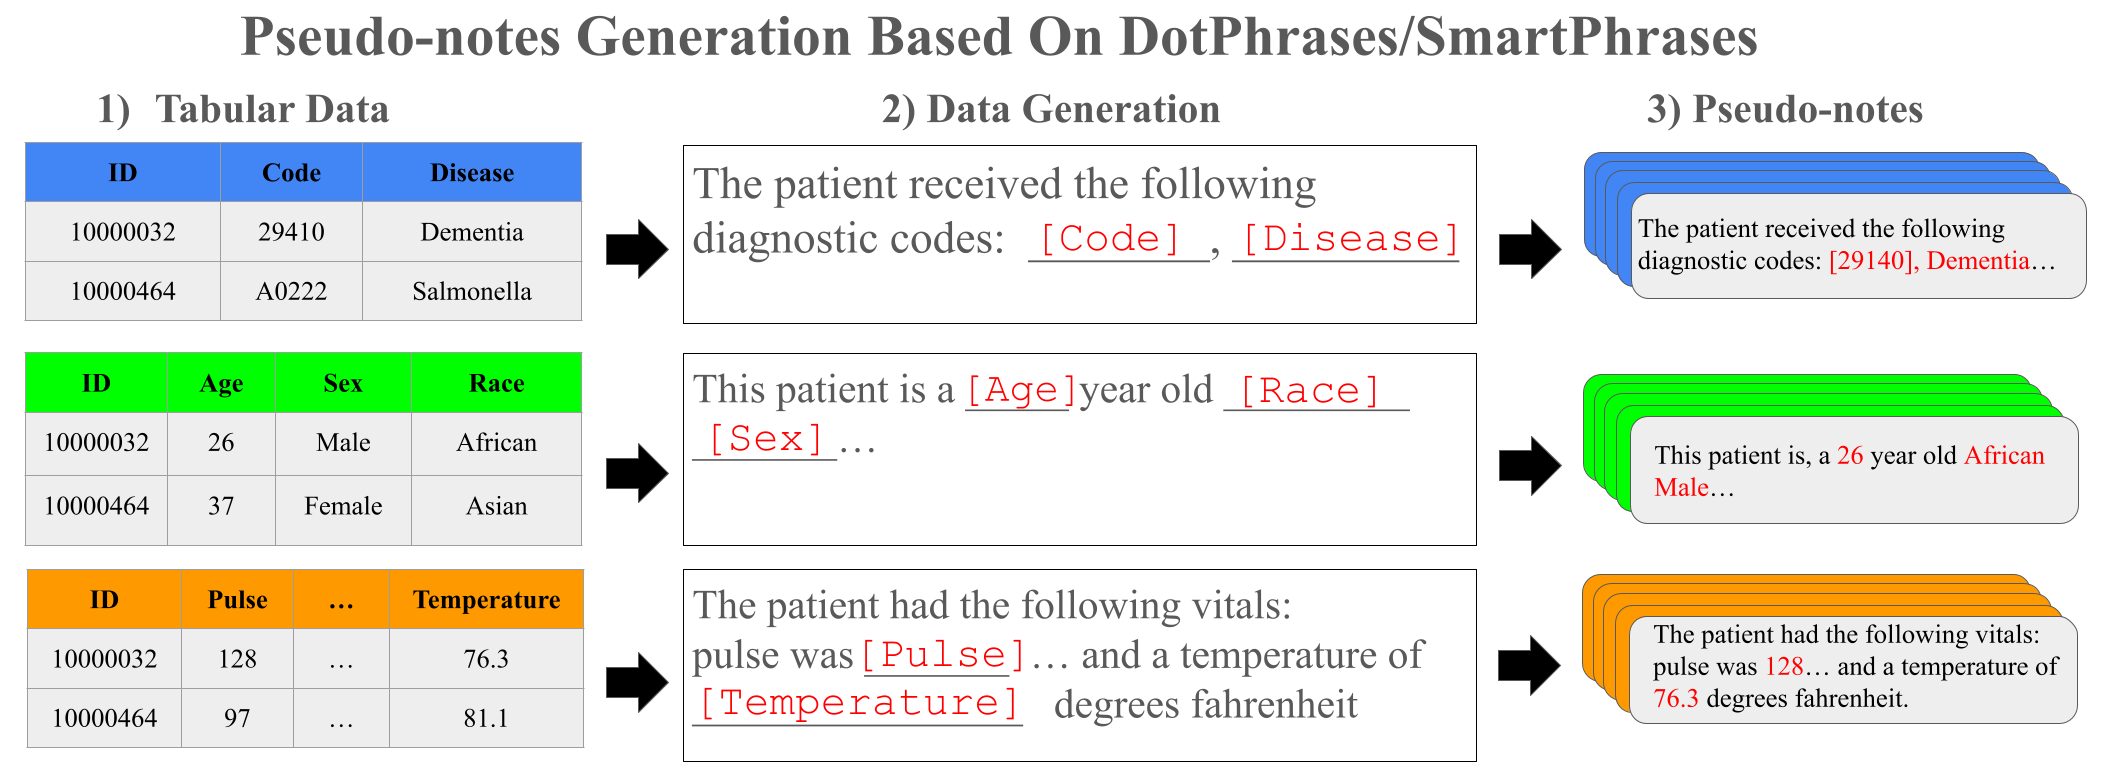
\includegraphics[width=\textwidth]{pseudo.png} 
   \caption{An Overview of Clinical Pseudo-Notes Generation: From Tabular Data to Text Using DotPhrases/SmartPhrases Commonly Employed in Healthcare.}
   \label{fig11} 
    \vspace*{-0.5cm}
 \end{figure} 
We begin by detailing the pseudo-notes method, which was developed in collaboration with a clinical informaticist at our institution. Although various approaches for text generation using Large Language Models (LLMs) have been explored \citep{hegselmann2024data} \citep{ellershaw2024automated}, we identify potential pitfalls in current methodologies due to issues related to hallucinations, as described in \citep{hegselmann2024data} and \citep{lee2024large}. To address these challenges, we employ a more traditional serialization process mimicking SmartPhrases/DotPhrases on the Epic
EHR system \citep{chang2021emr}, which assists in accurately filling in relevant clinical information within a fixed passage to generate the pseudo-notes as shown in Figure \ref{fig11}. We construct separate notes for each clinical modality (e.g., arrival, triage, etc.), resulting in six paragraphs for each patient visit. Additionally, we omit any patient identifiers within the text to mitigate the risk of overfitting on these unique identifiers (e.g., Patient ID, Hospital Admission ID, etc.). While there may be concerns surrounding the similarity between texts, we find that running a BERTopic \citep{grootendorst2022bertopic}, which is analogous to Latent Dirichlet Allocation (LDA), finds unique topics within our corpus of pseudo-notes text. Example Pseudo-notes are attached in the Appendix (\ref{exnotes}).
% We showcase this in Figure 2.

\subsection{Multiple Embedding Model for EHR (MEME) Architecture}
In this section, we outline our model architecture, which is crucial to our end-to-end pipeline. These networks are tailored to process preprocessed and tokenized textual inputs, outputting logits for each class. The class with the highest probability is then selected as the predicted class. We begin by explaining that this approach is designed to embed a patient's modalities separately, accommodating the variable textual lengths associated with different patient visits as described in \citep{rupp_exbehrt_2023}. This strategy addresses a limitation of the BERT architecture, which has a sequence limit of 512 tokens. This method is preferable to the truncation involved in fitting all text into a single heterogeneous embedding, as it better preserves the integrity of the input data and it omits any concerns regarding different ordering strategies. A direct comparison of these approaches can be seen in Figure \ref{arc} which shows our proposed architecture (MEME) over the conventional single heterogenous embedding approach (MSEM).

\begin{figure}[t]
   \centering 
   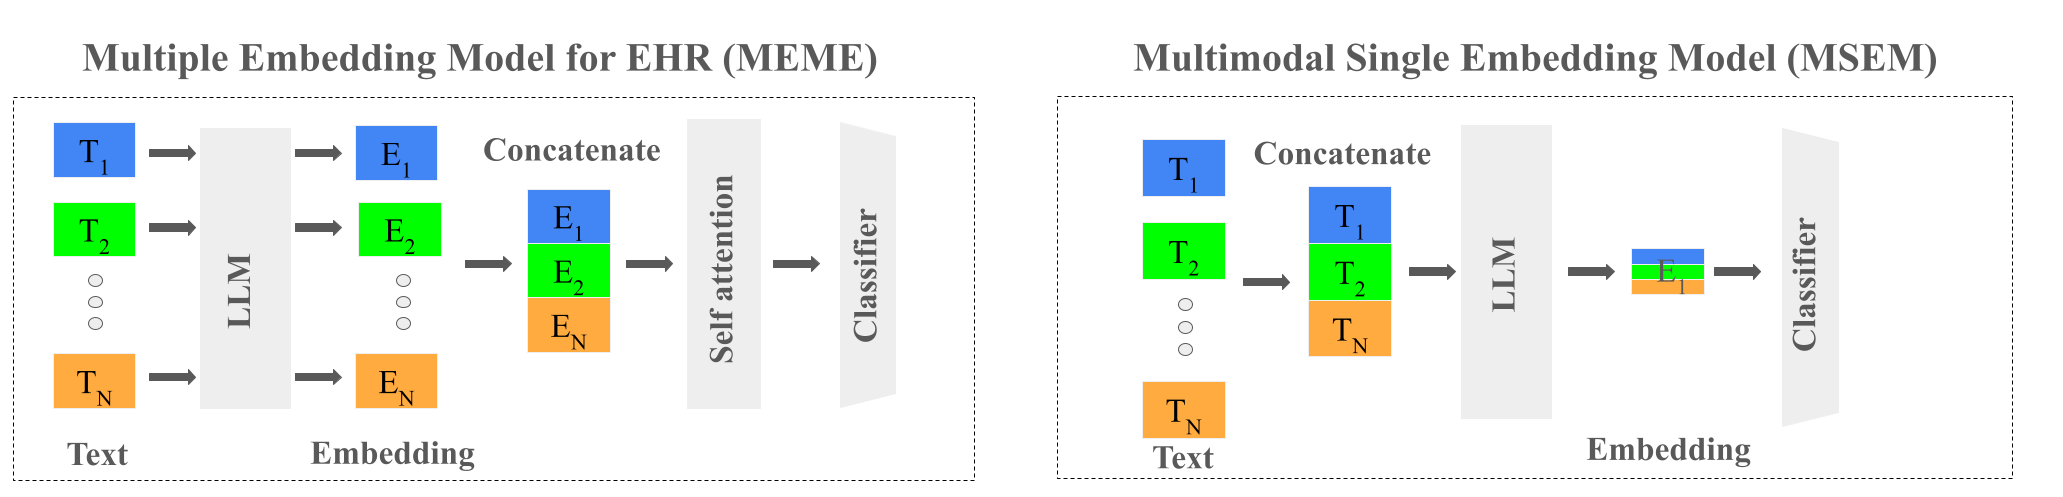
\includegraphics[width=\textwidth]{arc.png} 
   \caption{The Multiple Embedding Model for EHR (MEME) and the Multimodal Single Embedding Model (MSEM) side by side.}
   \label{arc} 
    \vspace*{-0.5cm}
 \end{figure} 

\subsubsection{Step 1: Generating Embeddings}

In the initial step of our model, we aim to generate embeddings for each EHR concept by feeding tokenized data into our foundational models' encoders, which produce rich, high-dimensional vector representations encapsulating various aspects of a patient's medical history. We choose to freeze the encoder layers, focusing on the training parameters of the subsequent layers dedicated to the prediction task. After generating embeddings for all concepts, we concatenate them into a unified input vector for further processing. This procedure can be mathematically represented as follows: In the model's first phase, modality-specific pseudo-notes are processed and structured into a tokenized format, denoted $D_{\text{tokenized}}$, which outlines a series of unique medical concepts or characteristics ($c_i$) derived from a patient's records. Each concept undergoes transformation via the foundation models' encoder into a high-dimensional vector $\vec{v}_i$, capturing clinical information via context-rich portrayals of each EHR concept. These vectors are then unified into a comprehensive vector $\vec{V}_{\text{concat}}$ through concatenation, laying the groundwork for our multimodal patient embeddings.

\begin{equation}
    \vec{v}_i = \text{FoundationModel}(c_i) \quad \forall c_i \in D_{\text{tokenized}}
\end{equation}
\begin{equation}
    \vec{V}_{\text{concat}} = \text{Concatenate}(\vec{v}_1, \vec{v}_2, \ldots, \vec{v}_n)
\end{equation}

\subsubsection{Step 2: Self-attention Classifier}

In the second step of our network, we introduce a new use case of a self-attention layer \citep{vaswani2017attention} designed to analyze the singular concatenated representation vector, $\vec{V}_{\text{concat}}$, as a unified entity. This approach arises from our intention to interpret aligned modalities collectively, rather than as separate entities, allowing the network to operate comprehensively on the entire vector. It evaluates the relationships between elements within the vector, capturing patterns across different EHR concept vectors. 
% We motivate this method by training a basic self-attention layer from scratch within the feed-forward network, focusing on updating the gradients of this specific component. 
The output from this layer is then directed through a fully connected layer, followed by a ReLU activation function, before being fed into the final classifying layer for prediction. This method, characterized by a unified analysis and attention-based processing, distinguishes our approach from traditional models and is pivotal to the enhanced predictive capabilities of our framework. Mathematically, this process involves transforming the input vector $\vec{V}_{\text{concat}}$ into an attention vector $\vec{V}_{\text{attention}}$ using the self-attention mechanism, further processing it through a fully connected (FC) layer and a Rectified Linear Unit (ReLU) activation to obtain a refined feature vector $\vec{V}_{fc}$, as outlined below:

\begin{equation}
    \vec{V}_{\text{attention}} = \text{SelfAttention}(\vec{V}_{\text{concat}})
\end{equation}
\begin{equation}
    \vec{V}_{fc} = \text{ReLU(FC}(\vec{V}_{\text{attention}}))
\end{equation}
\begin{equation}
    \vec{z} = \text{Classifier}(\vec{V}_{fc})
\end{equation}

The model leverages these refined features, $\vec{V}_{fc}$, in a classifier to produce logits $\vec{z}$, subsequently processed to predict probabilities for ED Disposition or ED Decompensation tasks. The classifier's output is optimized by minimizing Cross Entropy Loss $L$, ensuring alignment of predicted probabilities $\hat{y}$ with true labels $y_i$. For multi-label tasks like ED Decompensation, each logit $\vec{z}_{i,l}$ undergoes individual sigmoid activation $\sigma$, and the model's training involves minimizing a tailored Cross Entropy Loss that aggregates binary cross-entropy losses across all labels for each observation, capturing the multi-label aspects of the data effectively.

% \subsection{Foundation Model Selection}

% We evaluate five different BERT-based models, as well as two other large language models, as potential foundation model backbones for our task, assessing their embedding quality and generalization capabilities. The models under consideration are shown in Table \ref{TableModel} with descriptions for each model. We elected to utilize a BERT-based approach due to its bidirectional embeddings, which provide a more complete view of the context around each word. This allows better reasoning about a word's meaning and role for prediction tasks like the ones presented in this work. In contrast, GPT's left-to-right embeddings may miss important contextual cues from future words, limiting their effectiveness for many prediction tasks that require joint understanding of the full context (\citep{ethayarajh2019contextual}, \citep{schomacker2021language}, \citep{topal2021exploring}).

% The foundation model backbones are evaluated for their effectiveness and generalization capabilities on our specific ED Disposition task, with the goal of selecting the most suitable option for our use case which we will later highlight as the multiple embedding model for EHR (MEME). The results are displayed in Figure \ref{fm}. From this analysis we find Medbert \citep{9980157} which was built on top of \citep{alsentzer2019publicly} to be the most suitable foundation model.

%  \begin{figure}[t]
%    \centering 
%    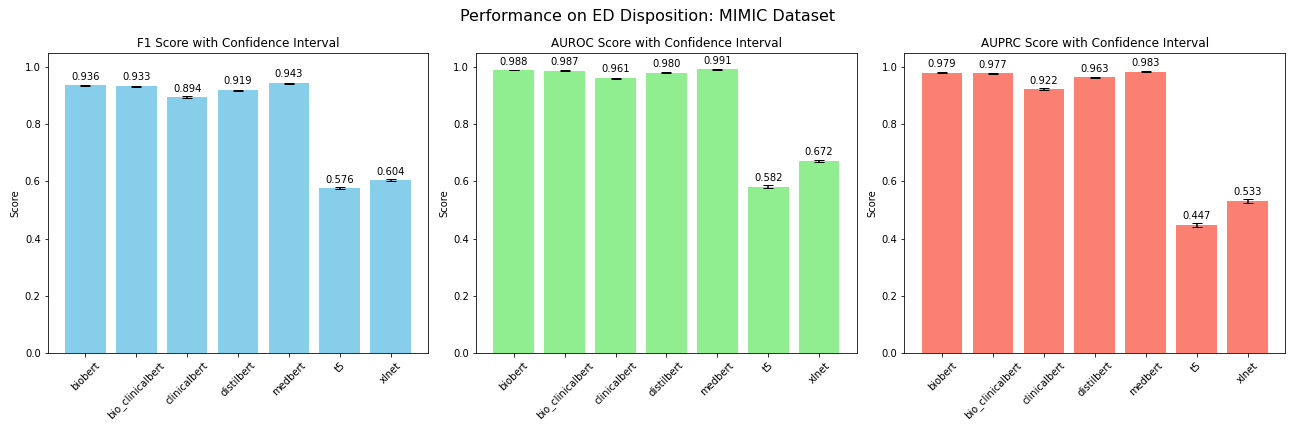
\includegraphics[width=\textwidth]{fm_eval.png} 
%     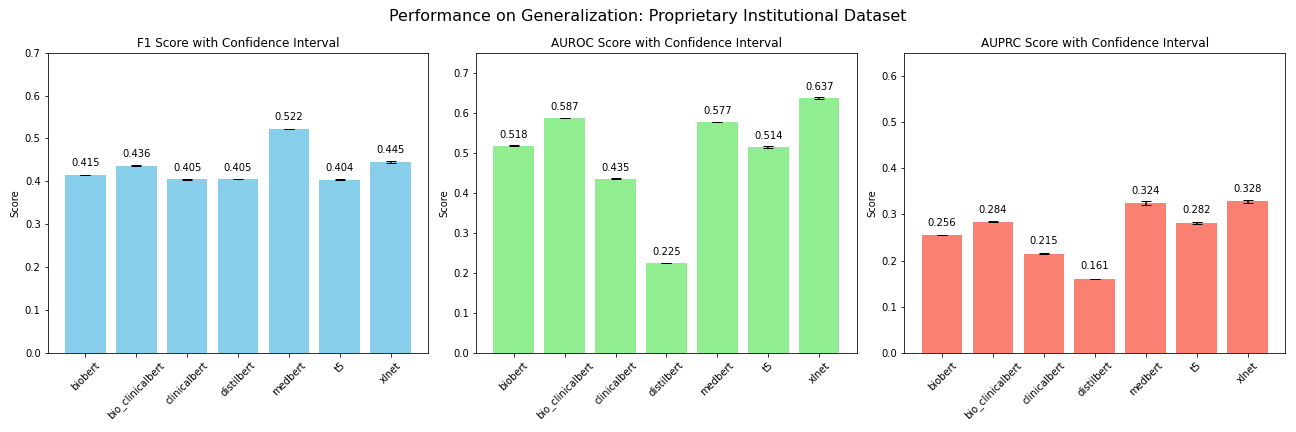
\includegraphics[width=\textwidth]{generalize.png} 
%    \caption{The benchmark of various foundation models evaluated on ED Disposition. We also explore the model that best generalizes with an additional proprietary instutional dataset for foundation model selection. However as displayed, all models have trouble with Generalization.}
%    \label{fm} 
%  \end{figure} 

\subsection{Preprocessing \& Model Optimization}
\subsubsection{{Missing data imputation and tokenization}} %Preprocessing}

\iffalse{Our data curation process begins by constructing pseudo-notes from our raw EHR data. Initially, we disregard missing entries in the tabular format during the conversion from tabular to text.}\fi {Tabular EHR are converted into pseudo-notes using predefined templates as described above.} {To represent missing data entries, we incorporate} \iffalse{Subsequently, we address the missing data by incorporating} \fi filler sentences such as \texttt{"The patient did not receive any medications"} in cases where the medication reconciliation (medrecon) modality data is missing. We apply this method to all six modalities before feeding them into our tokenizer derived from the MedBERT model. This model utilizes a subword tokenizer optimized to handle out-of-vocabulary (OOV) words by segmenting words into smaller subword tokens or subword pieces, with a vocabulary size of 28,996 subword tokens. We then split our dataset into training, validation, and testing sets using a fixed seed to ensure the replicability of the results found in this study, thus concluding the data preprocessing phase.

\subsubsection{Model Optimization}

The models were trained with a batch size of 64, a dropout rate of 0.3, the AdamW optimizer with a learning rate of 5e-5, and a linear learning rate scheduler. For the ED disposition task, we employed Cross-Entropy Loss, and for multilabel decompensation classification, we used Binary Cross-Entropy (BCE) Loss. Training proceeded until a minimum was reached in the validation loss across 10 epochs with early stopping implemented. We tracked F1 scores and loss after each epoch to assess the model's effectiveness. Our computational framework was developed in Python's PyTorch, using large language models available on the HuggingFace \citep{wolf2019huggingface} Platform. For development purposes, we utilized the g4dn.4xlarge EC2 instance from AWS Cloud Services. The model's training and testing were conducted on a single Tesla V100 GPU with 16GB of VRAM to ensure efficient processing.


% Tell us your techniques!  If your paper is develops a novel machine
% learning method or extension, then be sure to give the technical
% details---as you would for a machine learning publication---here and,
% as needed, in appendices.  If your paper is developing new methods
% and/or theory, this section might be several pages.

% If you are combining existing methods, feel free to cite other
% packages and papers and tell us how you put them together; that said,
% the work should stand alone for someone in that general machine
% learning area.  

% \emph{Lack of technical details, such that the soundness of the
%   methods can be verified, is a major reason that otherwise
%   strong-looking papers are scored low/rejected.}

\section{Results}

% overview

\subsection{Model optimization}

% we used ED disposition as teh reference task for selecting the best backbone

\subsubsection{Embedding Model Selection}

 \begin{figure}[h!]
   \centering 
   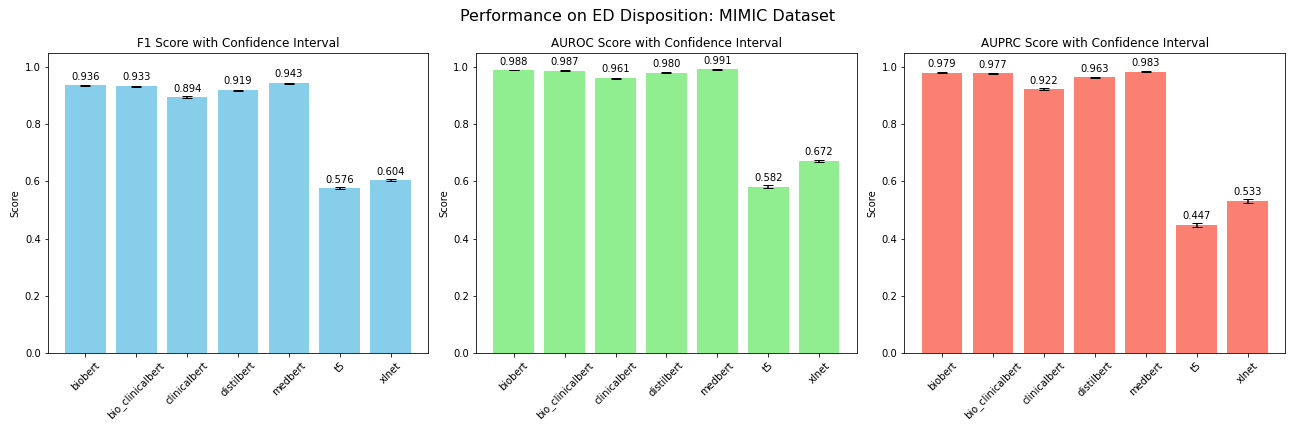
\includegraphics[width=\textwidth]{fm_eval.png} 
    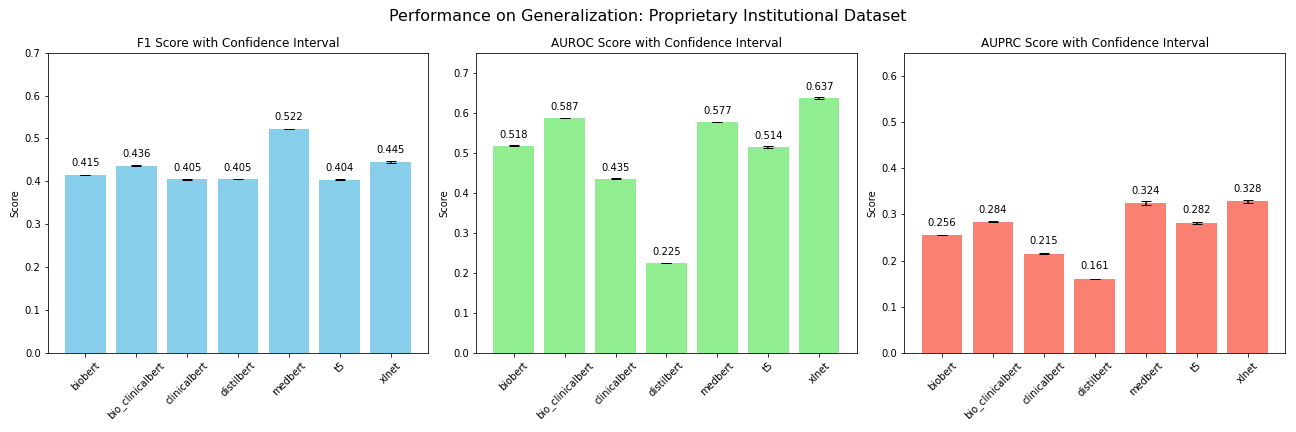
\includegraphics[width=\textwidth]{generalize.png} 
    \vspace*{-0.5cm}
   \caption{The benchmark of various foundation models evaluated on ED Disposition. We also explore the model that best generalizes with an additional proprietary institutional dataset for foundation model selection. However, as displayed, all models have trouble with generalization.}
   \label{fm} 
 \end{figure} 
\vspace*{-0.5cm}

We evaluate five different BERT-based models, as well as two other large language models, as potential foundation model backbones for our task, assessing their embedding quality and generalization capabilities. The models under consideration are shown in Appendix Section (\ref{model_des}) in Table \ref{TableModel} with descriptions for each model. We elected to utilize a BERT-based approach due to its bidirectional embeddings, which provide a more complete view of the context around each word. This allows better reasoning about a word's meaning and role for prediction tasks like the ones presented in this work. In contrast, GPT's left-to-right embeddings may miss important contextual cues from future words, limiting their effectiveness for many prediction tasks that require joint understanding of the full context (\cite{ethayarajh2019contextual}; \cite{schomacker2021language}; \cite{topal2021exploring}).

The foundation model backbones are evaluated for their effectiveness and generalization capabilities on our specific ED Disposition reference task, with the goal of selecting the most suitable option for our use case as the multiple embedding model for EHR (MEME). The results are displayed in Figure \ref{fm}. From this analysis we find Medbert \citep{9980157}, which was built on top of \citep{alsentzer2019publicly}, to be the most suitable foundation model.

% \subsection{Ablation Study: Advantages of Multimodal Data \& MEME Approach}
\subsubsection{Multimodal vs unimodal EHR representation}

\begin{figure}[h!]
   \centering 
   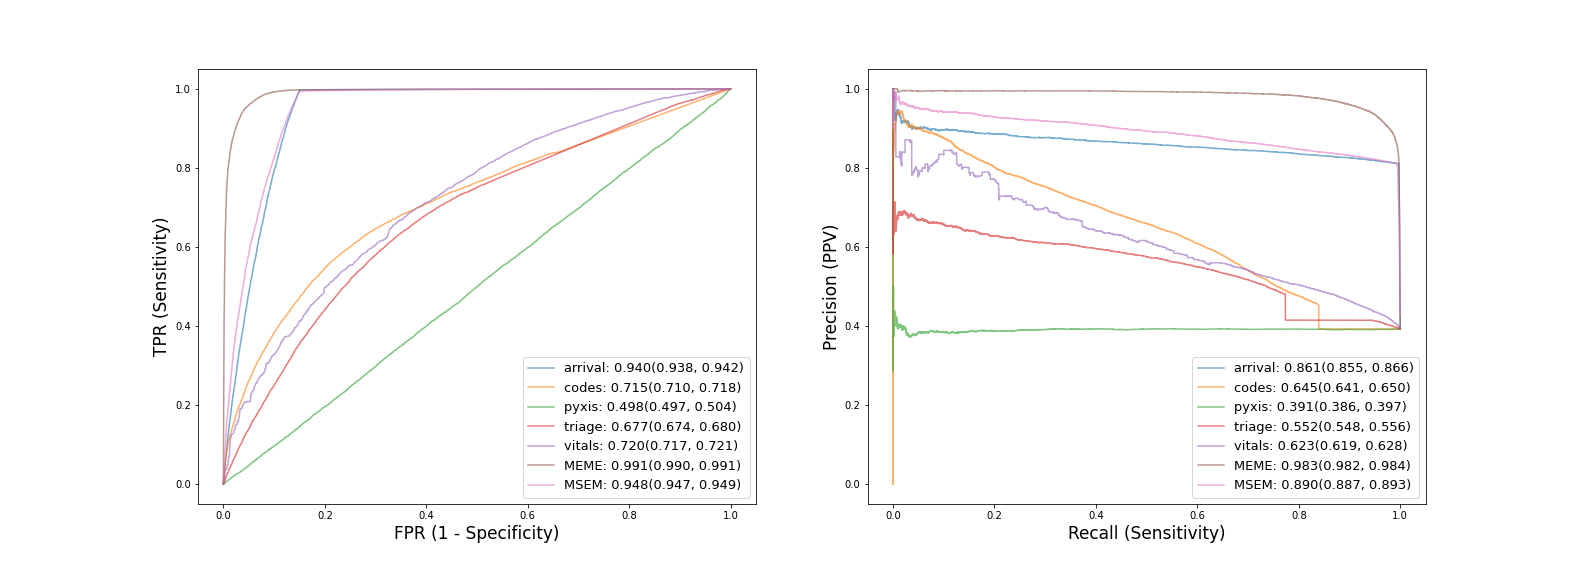
\includegraphics[width=\textwidth]{results.png} 
   \vspace*{-0.5cm}
   \caption{We performed an ablation study where each modality was used alone to predict the ED Disposition reference task, showcasing the added value of a multimodal data approach.}
   \label{abs} 
 \end{figure} 
\vspace*{-0.5cm}
We conduct an ablation study to highlight the benefits of adopting a multimodal data and multiple embedding approach, as illustrated in Figure \ref{abs}. Further results tables can be seen in Appendix Section (\ref{ablation}). This analysis allows us to identify which modalities are most indicative of predicting Emergency Department Disposition based on sets of AUROC and AUPRC results. We observe that no single modality on its own can outperform MEME, as demonstrated through direct comparisons. Additionally, we benchmark MEME against a model designed to encapsulate all multimodal information within a single, heterogeneous embedding. We find that this model's predictive capability is somewhat diminished which is consistent with \citep{rupp_exbehrt_2023} due to truncation and sequence length limitations. This comparison further supports our decision to employ a multiple embedding strategy.

\subsection{MEME vs. reference models}

In our study, we evaluate the performance of the Multiple Embedding Model for EHR (MEME) against methodologies established by previous research \citep{xie2022benchmarking}, within the domain of Emergency Medicine. This benchmarking study informed comparing various frameworks  previously worked on in the literature as previous state of the art in Emergency Medicine analyses in the case of binary classification. In addition we included several benchmarks from related studies, adopting the methodology of their framework for our tasks.

% \begin{enumerate}
    % \item \textit{Logistic Regression}: Chosen for its simplicity and efficiency in binary classification tasks. Its interpretability and straightforward implementation make it a foundational tool for statistical analysis and machine learning, especially when working with binary or dichotomous outcomes.
    % \item \textit{Random Forest Classifier}: Selected for its interpretability and effectiveness with canonically tabular data, this model facilitates the evaluation of our text-conversion methodology.
    
    % \item \textit{Multi-Layer Perceptron (MLP)}: Chosen for its proficiency in handling high-dimensional tabular data, demonstrating versatility in model application.

    % \item \textit{GenHPF} \citep{hur2023genhpf}: This specialized model leverages the SimCLR framework for self-supervised learning of representations to predict outcomes. \textit{We keep in mind that this method utilizes all the available data from the MIMIC III, MIMIC-IV, and eICU datasets to form predictions.}

    
    % \item \textit{EHR-Shot} \citep{wornow2024ehrshot}: Utilizes the CLMBR-T Base Transformer, as proposed by \citep{steinberg2021language}, to generate patient representations from structured electronic health records (EHR) data, sourced from JSON files. These representations are subsequently employed to pursue our classification objectives, mirroring the strategy used in MEME.
    
    % \item \textit{MC-BEC} \citep{chen2023multimodal}: Adopts the model architecture outlined by Chen et al., which employs embeddings generated from multiple foundational models (\citep{huang2019clinicalbert}, \citep{yan2022radbert}). These embeddings are then used in a Light Gradient Boosting Model (LGBM) for prediction.
    
    % \item \textit{Multimodal Single Embedding Model (MSEM)}: Investigates the value of multimodal representation by concatenating all EHR modalities text and fitting it into a single embedding, as opposed to embedding them separately.

    % maybe add GPT here too, and note that we tested on a random subset (with asterisk in the table) 
% \end{enumerate}

These comparisons were run within and across datasets. The metrics used for evaluation include the F1 scores, the Area Under the Receiver Operating Characteristic Curve (AUROC), and the Area Under Precision-Recall Curve (AUPRC). To ensure robustness, 95\% confidence intervals were generated for each metric by resampling the test set 1,000 times. Our results—comprised of F1 scores, AUROC scores, and AUPRC scores—are presented in Tables (\ref{r1}, \ref{r2},  \ref{r3}).

% \subsection{MEME Outperforms Models}

\subsubsection{MEME vs traditional ML}
We observed that MEME {generally} surpasses the performance of {traditional techniques operating upon tabular EHR {Tables \ref{r1}, \ref{r2}, \ref{r3}}. We evaluated MEME against a logistic regression, random forest, and neural network model proposed on a previous benchmark \citep{xie2022benchmarking}, operating over tabular EHR prior to pseudonote generation.} \iffalse {the tabular Random Forest model and MLP. } \fi Although the Random Forest exhibits a competitive advantage in its AUROC, the imbalanced nature of these tasks makes the benchmarking more nuanced, as it performs inadequately under AUPRC \citep{saito2015precision}.

\subsubsection{MEME vs EHR foundation models}

{EHR-specific foundation models have been recently developed and have shown predictive capabilities across a variety of healthcare applications. We selected the following reference EHR FMs:}

\begin{enumerate}
    \item \textit{GenHPF} \citep{hur2023genhpf}: This specialized model leverages the SimCLR framework for self-supervised learning of representations to predict outcomes. \footnote{\textit{We keep in mind that this method utilizes all the available data from the MIMIC III, MIMIC-IV, and eICU datasets to form predictions while our method only uses that within the MIMIC-IV ED.}}

    
    \item \textit{EHR-Shot} \citep{wornow2024ehrshot}: Utilizes the CLMBR-T Base Transformer, as proposed by \citep{steinberg2021language}, to generate patient representations from structured electronic health records (EHR) data, sourced from JSON files. These representations are subsequently employed to pursue our classification objectives, mirroring the strategy used in MEME.
    
    \item \textit{MC-BEC} \citep{chen2023multimodal}: Adopts the model architecture outlined by Chen et al., which employs embeddings generated from multiple foundational models (\cite{huang2019clinicalbert}; \cite{yan2022radbert}). These embeddings are then used in a Light Gradient Boosting Model (LGBM) for prediction.
\end{enumerate}
We observed that MEME outperformed  MSEM, MC-BEC, EHR-shot models \footnote{The authors have noted that their CLMBR-t transformer does not support non-OMOP vocabulary contained in the MIMIC-IV database, potentially affecting its performance. We highlight this as a limitation in their EHR-shot model.} in this evaluation. We observe that GenHPF outperforms MEME in the AUROC metric, which can be directly compared with our method. However, it is worth mentioning that their approach incorporates all available EHR data from three databases (MIMIC III, IV, \& eICU) to inform these predictions, and thus test set signal may have leaked into the available model weights. Additionally, it is important to note that AUROC alone may not adequately reflect true performance, particularly in the context of our imbalanced classification objectives.

\begin{table}[H]
\caption{Benchmark study F1. A * denotes that the model operated on tabular data, and a $\dagger$ denotes the model operated on textual (pseudo-notes) data.}
\label{r1}
\begin{adjustbox}{width=\textwidth}
\begin{small}
\begin{tabular}{l|c|ccc}
\toprule
F1 Benchmark & Dispositon & & Decompensation &\\
Model & ED Disposition & Discharge & ICU & Mortality \\
\midrule
Logistic Regression (Baseline) * &0.799 $\pm$ 0.025&0.549 $\pm$ 0.033& 0.427 $\pm$ 0.036& 0.095 $\pm$ 0.026\\
Random Forest (Baseline) * & 0.826 $\pm$ 0.013 & 0.625 $\pm$ 0.026 & 0.544 $\pm$ 0.048 &  \textbf{0.175 $\pm$ 0.094}  \\
MLP * & 0.841 $\pm$ 0.010 & 0.612 $\pm$ 0.013 & 0.502 $\pm$ 0.019 & 0.097 $\pm$ 0.023 \\
GenHPF \citep{hur2023genhpf} * & --- & --- & ---& --- \\
EHR-Shot\citep{wornow2024ehrshot} *& 0.874 $\pm$ 0.003 & 0.691 $\pm$ 0.008 & 0.560 $\pm$ 0.008 & 0.036 $\pm$ 0.003 \\
MC-BEC\citep{chen2023multimodal} $\dagger$ & 0.912 $\pm$ 0.002& 0.653 $\pm$ 0.006 & 0.545 $\pm$ 0.006 & 0.127 $\pm$ 0.014\\
GPT3.5-turbo $\dagger$ & 0.764 $\pm$ 0.000& --- & --- & ---\\
MSEM $\dagger$& 0.893 $\pm$ 0.003 & 0.622 $\pm$ 0.007 & 0.334 $\pm$ 0.008 & 0.072 $\pm$ 0.014\\
MEME $\dagger$& \textbf{0.943 $\pm$ 0.003} & \textbf{0.698 $\pm$ 0.007} & \textbf{0.572 $\pm$ 0.014} & 0.137 $\pm$ 0.035 \\
\bottomrule
\end{tabular}
\end{small}
\end{adjustbox}
\end{table}
\vspace*{-0.5cm}
\begin{table}[H]
\caption{Benchmark study AUROC.}
\label{r2}
\begin{adjustbox}{width=\textwidth}
\begin{small}
\begin{tabular}{l|c|ccc}
\toprule
AUROC Benchmark & Dispositon & & Decompensation &\\
Model & ED Disposition & Discharge & ICU & Mortality \\
\midrule
Logistic Regression (Baseline) * &0.863 $\pm$ 0.012&0.852 $\pm$ 0.014 & 0.807 $\pm$ 0.017 & 0.768 $\pm$ 0.019\\
Random Forest (Baseline) *& 0.902 $\pm$ 0.010 & \textbf{0.862 $\pm$ 0.014} & \textbf{0.903 $\pm$ 0.016} &   0.847 $\pm$ 0.055\\
MLP *& 0.871 $\pm$ 0.018 & 0.802 $\pm$ 0.011 & 0.767 $\pm$ 0.011 & 0.786 $\pm$ 0.013 \\
GenHPF * & --- & 0.850 $\pm$ 0.000 & ---& \textbf{~0.870 $\pm$ 0.000} \\
EHR-Shot *& 0.790 $\pm$ 0.031 & 0.743 $\pm$ 0.007 & 0.821 $\pm$ 0.18 & 0.827 $\pm$ 0.009\\
MC-BEC $\dagger$& 0.968 $\pm$ 0.002 & 0.708 $\pm$ 0.006 & 0.818 $\pm$ 0.014 & 0.815 $\pm$ 0.006 \\
MSEM$\dagger$& 0.948 $\pm$ 0.002 & 0.552 $\pm$ 0.008 & 0.522 $\pm$ 0.009 & 0.546 $\pm$ 0.023\\
MEME $\dagger$& \textbf{0.991 $\pm$ 0.001} & 0.799 $\pm$ 0.006 & 0.870 $\pm$ 0.015 & \textbf{0.862 $\pm$ 0.006} \\
\bottomrule
\end{tabular}
\end{small}
\end{adjustbox}
\end{table}
\vspace*{-0.5cm}
\begin{table}[H]
\caption{Benchmark study AUPRC.}
\label{r3}
\begin{adjustbox}{width=\textwidth}
\begin{small}
\begin{tabular}{l|c|ccc}
\toprule
AUPRC Benchmark & Dispositon & & Decompensation &\\
Model & ED Disposition & Discharge & ICU & Mortality \\
\midrule
Logistic Regression (Baseline) * &0.874 $\pm$ 0.027&0.628 $\pm$ 0.036& 0.618 $\pm$ 0.034& 0.051 $\pm$ 0.034\\
Random Forest (Baseline) *& 0.902 $\pm$ 0.012 & 0.645 $\pm$ 0.036 & 0.571 $\pm$ 0.047 &  0.102 $\pm$ 0.044  \\
MLP *& 0.866 $\pm$ 0.018 & 0.630 $\pm$ 0.024 & 0.581 $\pm$ 0.026 & 0.077 $\pm$ 0.033 \\
GenHPF * & --- & --- & ---& ---   \\
EHR-Shot *& 0.878 $\pm$ 0.007 & 0.655 $\pm $ 0.012 & 0.655 $\pm$ 0.017 & \textbf{0.246 $\pm$ 0.030} \\
MC-BEC $\dagger$& 0.935 $\pm$ 0.003& 0.657 $\pm$ 0.009 & 0.608 $\pm$ 0.09& 0.174 $\pm$ 0.025 \\
MSEM $\dagger$& 0.890 $\pm$ 0.005 & 0.493 $\pm$ 0.010 & 0.216 $\pm$ 0.009 & 0.037 $\pm$ 0.006\\
MEME $\dagger$& \textbf{0.983 $\pm$ 0.002} & \textbf{0.765 $\pm$ 0.008} & \textbf{0.709 $\pm$ 0.012} & 0.243 $\pm$ 0.034 \\
\bottomrule
\end{tabular}
\end{small}
\end{adjustbox}
\end{table}

\subsubsection{MEME vs MSEM}
{Consistent with our prior analysis of multimodal EHR representation, we found that MEME significantly outperformed single-modality embedding (MSEM) across all tasks (Tables \ref{r1}, \ref{r2}, \ref{r3}). A primary rationale for the discrepancy between MEME and MSEM could be attributed to MedBERT's, and more generally BERT architectures', token sequence length, which truncates all input after reaching its 512-sequence limit.

\subsubsection{MEME vs LLM prompting}

\begin{figure}[h!]
    \centering
    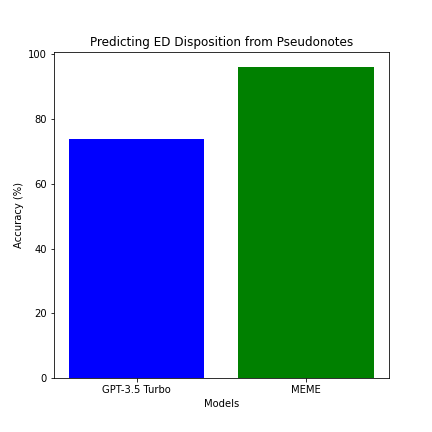
\includegraphics[width=2in]{dispo.png}
    \vspace*{-0.5cm}
    \caption{Comparison of Classification Accuracies: Training a Classifier (MEME) versus Utilizing a Generative Model (GPT-3.5-Turbo) for Prediction}
    \label{gpt-meme}
    \vspace*{-0.5cm}
\end{figure}
%rephrase

\iffalse {In addition to our benchmark, we address the question of whether training a classifier is essential, even with the emergence of generative AI models} \fi  {Given the emergent capabilities of generative AI models (e.g. GPT \citep{radford2018improving}, LLaMA-2 \citep{touvron2023llama}, Claude, etc.), we investigated predictive performance of MEME relative to a zero-shot prompting approach.} \iffalse {To explore this, we conducted a comparison between our} \fi {We compared the} MEME classifier and a zero-shot GPT-3.5-Turbo API using 100 random samples to predict ED disposition. Although our study's sample size is relatively small, we observed a performance gap displayed in Figure \ref{gpt-meme}, indicating that training a classifier remains preferable for accurate predictions. Even though GPT-3.5-Turbo exhibited performance beyond a random prediction, our findings underscore the continued importance of our approach.

% From Tables \ref{r1}, \ref{r2}, and \ref{r3}, it becomes evident that MEME outperforms all other models, including MSEM, MC-BEC, EHR-shot\footnote{The authors have noted that their CLMBR-t transformer does not support non-OMOP vocabulary contained in the MIMIC-IV database, potentially affecting its performance.}, as well as both baseline models (MLP and random forest classifiers). A primary rationale for the discrepancy between MEME and MSEM could be attributed to MedBERT's token sequence length, which truncates all input after reaching its 512-sequence limit. Additionally, it was observed that MEME surpasses the performance of the tabular Random Forest model and MLP. Although the Random Forest exhibits a competitive advantage in its AUROC, the imbalanced nature of these tasks makes the benchmarking more nuanced, as it performs inadequately when scrutinized through AUPRC. Furthermore, our method currently demonstrates superior performance compared to the standard medical events data models (EHR-shot) in these evaluations. This suggests that converting from a tabular to a textual format with MEME may yield a higher-quality representation of medical concepts, consequently enhancing task prediction performance and improving precision and recall.

% \subsection{Ablation Study: Advantages of Multimodal Data \& MEME Approach}

% \begin{figure}[h!]
%    \centering 
%    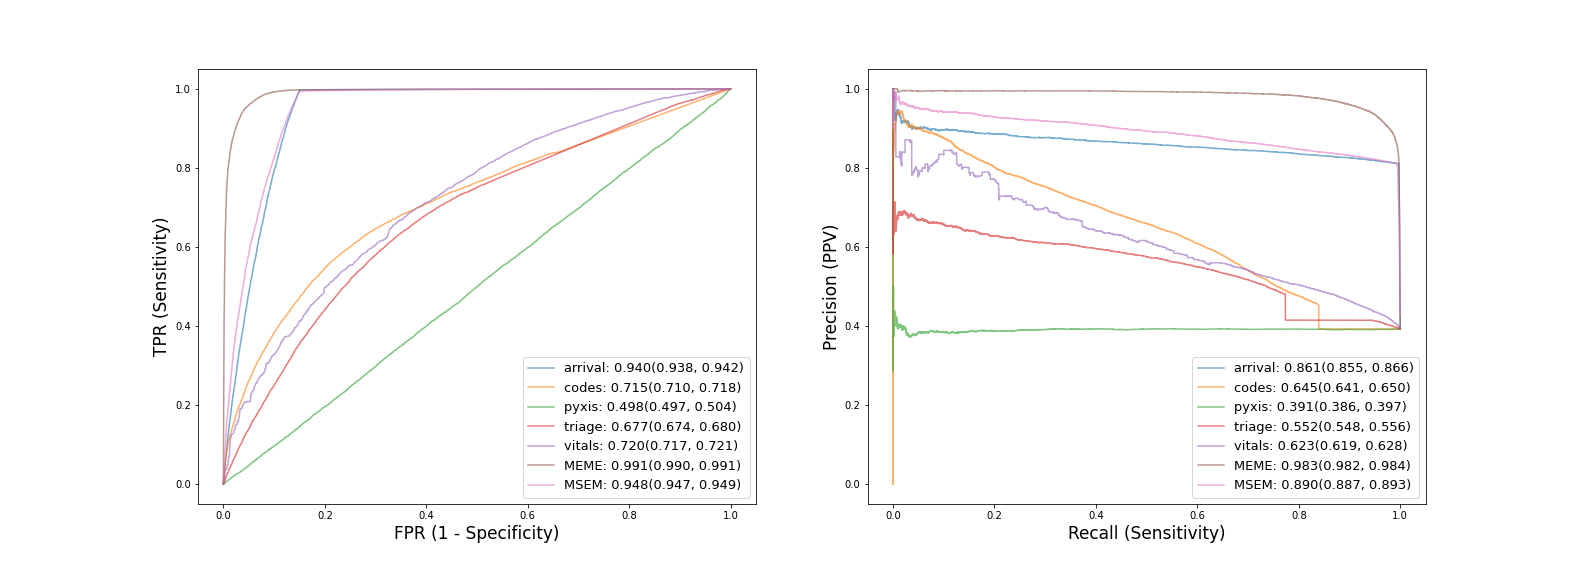
\includegraphics[width=\textwidth]{results.png} 
%    \caption{We performed an ablation study where each modality was used alone to predict the ED Disposition task, showcasing the added value of a multimodal data approach. We additionally included a multimodal method MSEM (Multiple Single Embedding Model) to demonstrate how a single heterogeneous embedding is affected by truncation indicated by its slightly declining performance, further motivating a multiple embedding approach.}
%    \label{abs} 
%  \end{figure} 

% We conduct an ablation study to highlight the benefits of adopting a multimodal data and multiple embedding approach, as illustrated in Figure \ref{abs}. This analysis allows us to identify which modalities are most indicative of predicting Emergency Department Disposition based on sets of AUROC and AUPRC results. We observe that no single modality on its own can outperform MEME, as demonstrated through direct comparisons. Additionally, we benchmark MEME against a model designed to encapsulate all multimodal information within a single, heterogeneous embedding. We find that this model's predictive capability is somewhat diminished due to truncation and sequence length limitations. This comparison further supports our decision to employ a multiple embedding strategy.

% \subsection{Is any of this necessary in the emergence of Generative AI?}

% \begin{figure}[h!]
%     \centering
%     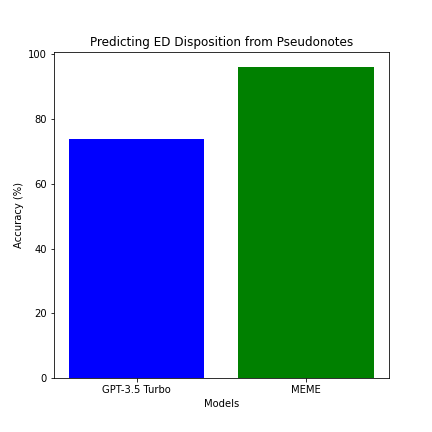
\includegraphics[width=2in]{dispo.png}
%     \caption{Comparison of Classification Accuracies: Training a Classifier (MEME) versus Utilizing a Generative Model (GPT-3.5-Turbo) for Prediction}
%     \label{gpt-meme}
% \end{figure}

% In addition to our benchmark, we address the question of whether training a classifier is essential, even with the emergence of generative AI models (e.g. GPT, LLaMA-2, Claude, etc.). To explore this, we conducted a comparison between our MEME classifier and a zero-shot GPT-3.5-Turbo API using 100 random samples to predict ED disposition. Although our study's sample size is relatively small, we observed a performance gap displayed in Figure \ref{gpt-meme}, indicating that training a classifier remains preferable for accurate predictions. Even though GPT-3.5-Turbo exhibited performance beyond a random prediction, our findings underscore the continued importance of our approach.

\subsection{Generalizability of our Method}

A recent critique of healthcare AI applications identified the lack of external validation and therefore potential overfitting to existing publicly available data. Indeed, we observed that while our approach and our reference models displayed strong within-dataset performance using a train-test split, performance was reduced when externally validated across institution (Figure \ref{bar13}).
These results are analogous to the study of \citep{jiang2023health}, who identified that fine-tuning on local hospital systems can improve general performance due to differences caused by demographics, locality, healthcare accessibility and more. 

\begin{figure}[h!]
\vskip 0.2in
\begin{center}
\label{bar}
\centerline{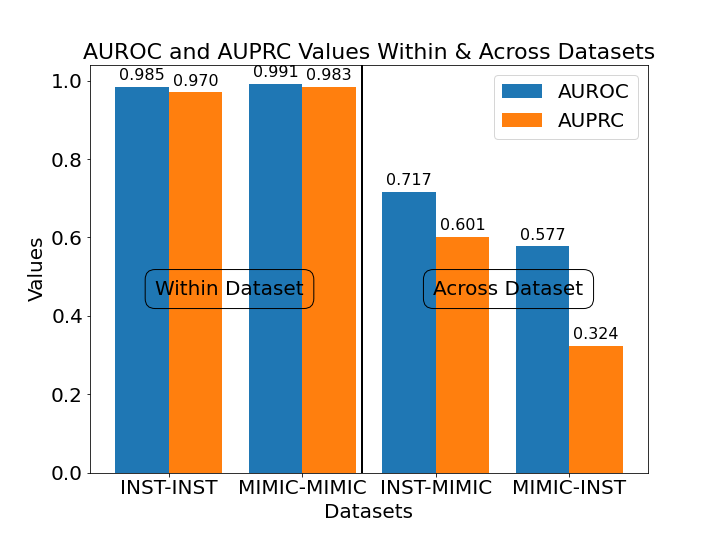
\includegraphics[width=4in]{bar2.png}}
\caption{Comparative Analysis of AUROC and AUPRC Values for Intra- and Inter-Dataset Evaluations: This bar chart illustrates the AUROC and AUPRC values of different models, where the models themselves are represented by their training and testing datasets (e.g., MIMIC-MIMIC). \textit{INST stands for institutional dataset}.}
\label{bar13}
\end{center}
\vskip -0.2in
\end{figure}

We performed a qualitative error analysis on the top 10 and bottom 10 scoring exemplars in our Institutional dataset to gain insight into this performance gap. Concordant cases were defined as those which the model scored highly and were correctly identified, or scored lowly and correctly not flagged, and Discordant cases were defined as vice versa. No systematic patterns or patient attributes were immediately apparent from investigating the decision making of this model in these groups, necessitating future study. \iffalse{We found no systematic patterns or attributes of patients that explained this gap.}\fi

However, we observed qualitative differences between datasets in terms of EHR features. {We compared the unique tabular values across the two EHR databases and observed only moderate overlap between values and concepts} \iffalse{We additionally explored the heterogeneity of the data inputs within our pseudonotes method, where we identified differences of unique values (i.e. Categorical - Venn Diagram, Numerical - Boxplots) from all the features across our two tabular EHR databases. We find that these results seen in Figure } \fi (Figure \ref{venn}). For a more detailed perspective see appendices (Section \ref{gener3}). This might reflect systematic differences in patient populations or hospital protocols. \iffalse{, appear to be behind this failed generalizability}\fi 

\begin{figure}[h!]
\vskip 0.2in
\begin{center}
\label{bar}
\centerline{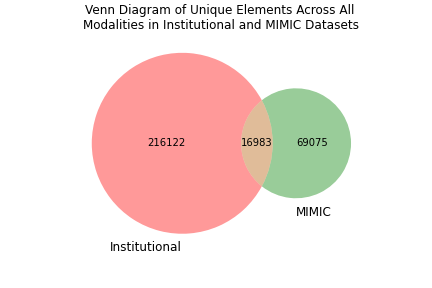
\includegraphics[width=4in]{plots/venn.png}}
\caption{Venn Diagram of Unique Features across all modalities respective of both EHR Systems. Note the large differences in features.}
\label{venn}
\end{center}
\vskip -0.2in
\end{figure}

\vspace*{-0.5cm}
% \emph{This section is optional, and more theoretical work may not need
%   this section.  However, if you are using health data, then you need
%   to describe it carefully so that the clinicians can validate the
%   soundness of your choices.} 

% Describe the cohort.  Give us the details of any inclusion/exclusion
% criteria, what data were extracted, how features were processed,
% etc.  Recommended headings include:

% \subsection{Cohort Selection} 
% This includes choice of criteria and basic numbers, as well as any relevant
% information about the study design (such how cases and controls were
% identified, if appropriate), 

% \subsection{Data Extraction} 
% This includes what raw information you extracted or collected, including any
% assumptions and imputation that may have been used, and 

% \subsection{Feature Choices} 
% This includes how you might have converted the raw data into features that were
% used in your algorithm. 

% Cohort descriptions are just as important as methods details and code
% to replicate a study.  For more clinical application papers, each of
% the sections above might be several paragraphs because we really want
% to understand the setting.

% For the submission, please do \emph{not} include the name of the
% institutions for any private data sources.  However, in the
% camera-ready, you may include identifying information about the
% institution as well as should include any relevant IRB approval
% statements.

% \subsection{Results on Synthetic Experiments}

% \emph{Depending on the claim you make in the paper, this section may
%   not be relevant.}

% Especially if you are developing a new method, you will want to
% demonstrate its properties on synthetic or semi-synthetic experiments.
% Include experiments that will help us understand the contribution of
% the work to machine learning and healthcare. 

% \section{Results on Real Data} 
\section{Discussion \& Conclusion}

In this paper we introduce \iffalse{our model MEME ,}\fi {a Multimodal Embedding Model for EHR (MEME), a representation framework for EHR. MEME is built upon two core concepts: 1) The text serialization of tabular EHR into pseudo-notes, which provides an interface with language foundation models; and 2) the multimodal framing of EHR to reflect the heterogeneity of the underlying data.} \iffalse{an approach for transforming multimodal tabular EHR data into clinical pseudo-notes. This transformation \iffalse{significantly}\fi enhances the interpretability of our data inputs and utility of EHR data in various healthcare-related tasks. The pseudo-notes method not only simplifies data handling but also effectively bridges the gap between traditional EHR formats and advanced NLP techniques employed in modern machine learning.} \fi
{We demonstrate that this combination outperforms traditional ML techniques, EHR-specific foundation models, and prompting-based approaches across decision support tasks in the Emergency Department.} \iffalse{A key finding from our study is the superior performance of the multimodal strategy employed by MEME. It  outperforms a traditional machine learning method, and other methods found in the literature, demonstrating the benefits of encoding different components of EHR separately. This approach allows for a more comprehensive representation of a patient's medical profile, capturing a broader spectrum of medical information crucial for accurate predictions. }\fi

{In addition to the performance advantages demonstrated by our experiments, MEME has several qualitative benefits in terms of portability and extendibility. EHR-specific models, such as BEHRT \citep{li_behrt_2020}, CHIRoN \citep{hill2023chiron}, EHR-shot \citep{wornow2024ehrshot}, etc., rely on data standards and transparent harmonization procedures to ensure interoperability, and their general applicability is severely hampered by the fact that these standards are still being developed and evaluated (e.g., MEDS\_ETL vs OMOP). It is also unclear how these models should be extended to accommodate new and updated medical concepts \citep{arnrich2024medical}. By contrast, the natural language approach is extendible to any data that can be text-serialized, which is more easily adopted by institutions, and can more gracefully handle changes in coding standards, all the while leveraging general reasoning capabilities and increasing medical domain knowledge captured by LLMs. While all of our findings were demonstrated within the Emergency Department setting, we hypothesize that they should generalize into other common decision support scenarios.}

% We expect that this approach is robust and extendible
%qualitative advantages of pseudo-notes in terms of portability:
% 1. smoother data processing; 2. extendible to clinical notes and other data types. 3. extendible to other tasks beyond ED)

% \subsection{Pseudo-notes is smoother for data processing}
% In terms of data handling and preparation, we found that our pseudo-notes method, from raw input to output, was more efficient and easier to handle compared to the benchmarked methods. These methods rely on the Medical Events Data Standard (MEDS\_ETL \citep{arnrich2024medical}), which is still under development. While the comparison of our approach isn't direct, since we are comparing a text based method to a tabular one, we still find this to be worth noting. We identified various issues and dataset limitations with meds\_etl at its current state primarily due to the hardcoding of file transformations within their pipeline. This hardcoding restricts their utility for proprietary (Institution) datasets and non hard-coded datasets (MIMIC-IV ED), where such specific information may not be available. Additionally, their CLMBR-T transformer does not support non-OMOP vocabularies, making it challenging to perform a direct comparison and benchmark of methods. 


% \subsection{JSON Generated Versus Pseudo-notes Method Comparisons}

% We conducted an analysis on the data generation process, comparing text generation via large language models (LLMs) to our pseudo-notes method. We found that inputting JSON data into LLMs like GPT-4 and LLaMA-2, which are not optimized for parsing structured tables, leads to a small degree of ``hallucination." This issue is particularly pronounced in long contexts, critically impacting the integrity of our original data. These findings are underscored in \citep{hegselmann2024data}. However, it's important to note the extensive efforts recently undertaken by groups such as LLaMA Index and detailed in recent studies (\citep{song2023restgpt}, \citep{jiang2023large}, \citep{chen2024beyond}, \citep{yao2023sai}) to mitigate this issue. Nonetheless, given the importance of accuracy and sensitivity in applications like healthcare, we argue that a fill-in approach may offer a more conservative and reliable alternative.




% However, our findings also highlight a significant challenge in the field of EHR analysis: the limited generalizability of models across different hospital institutions. Despite its strengths, the representation derived from the MIMIC-IV Database proved insufficient for generalization across diverse healthcare systems. This underscores the need for more representative publicly available datasets that can generalize to other EHR systems.

% \emph{Depending on the claim you make in the paper, different
%   components may be important for this section.}

% \subsection{Evaluation Approach/Study Design} 
% Before jumping into the results: what exactly are you evaluating?
% Tell us (or remind us) about your study design and evaluation
% criteria.

% \subsection{Results on Application A} 

% Present your numbers and be sure to compare proposed methods against appropriate baselines. 
% You should provide a summary of
% the results in the text, 
% as well as in tables (such as
% Table~\ref{tab:example}) and figures (such as
% Figure~\ref{fig:example}).  
% You may use subfigures/wrapfigures 
% so that figures don't have to span the whole page or multiple figures are side by side.

% \begin{table}[t]
%   \centering 
%   \caption{Description with the main take-away point. Note that the caption should appear \emph{above} the table.}
%   \begin{tabular}{llll}
%   \toprule
%     \textbf{Method} & \textbf{Metric1} & \textbf{Metric2} & \textbf{Metric3} \\
%     \midrule
%     Baseline & 1.1 & 2.3 & 0.1 \\ 
%     NetNet & 41.3 & 31.9 & 77.4 \\ 
%     \bottomrule
%   \end{tabular}
%   \label{tab:example} 
% \end{table}

%  \begin{figure}[t]
%    \centering 
%    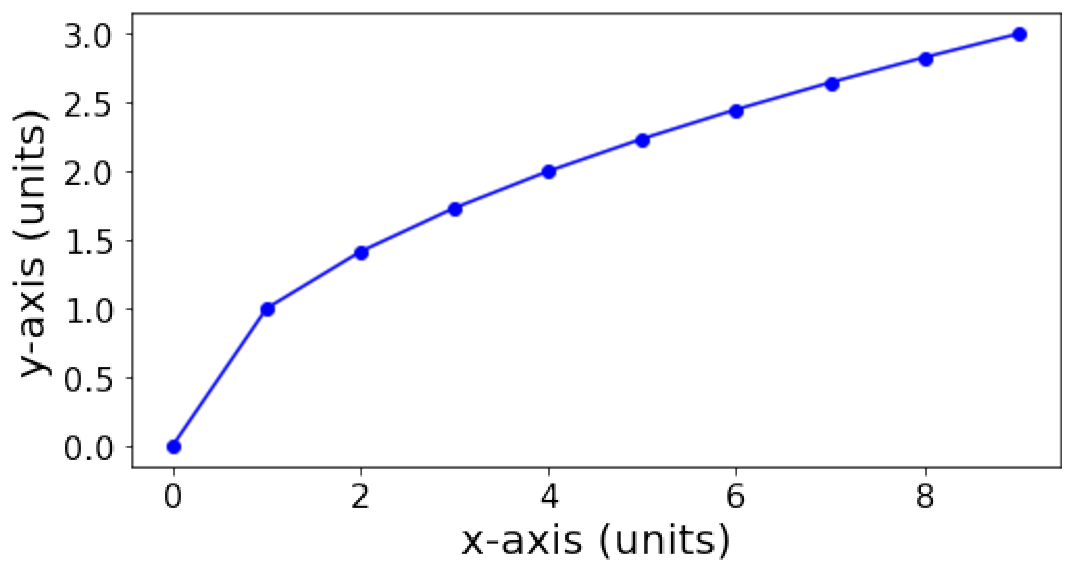
\includegraphics[width=2.5in]{plot.pdf} 
%    \caption{Description with the main take-away point. Note that figure captions should appear below the figure.}
%    \label{fig:example} 
%  \end{figure} 

% \subsection{Results on Application/Follow-up Study B} 

% \section{Required: Discussion} 

% \emph{This is probably the most important section of your paper!  This
%   is where you tell us how your work advances our understanding of
%   machine learning and healthcare.}  Discuss both technical and
% clinical implications, as appropriate\cite{xyz19}.

\paragraph{Limitations}

One crucial limitation of the model is the poorly performing external validity caused by the heterogenous nature of two EHR datasets. 
% While building a training dataset that combines MIMIC and our UCLA EHR, or performing external-site-specific fine tuning could alleviate this performance drop-off, it is important to highlight that different hospital systems may result in generalizability for this model and competitors, as identified by Wornow and colleagues \citep{wornow_shaky_2023}. 
We saw in our results that it is likely that protocols around patient care vary across site and over time such that the same patient would experience different outcomes depending on when and where they experienced care. Therefore we conclude that current models developed on the publicly available MIMIC-IV ED dataset appear to be insufficient for ensuring true generalization across diverse healthcare systems.

Another limitation of this work is our inability to release our private institutional data, due to privacy restrictions and university policy. This highlights the significance of independent benchmarks, and underscores the necessity of external validation, including benchmark datasets and tasks such as MC-BEC \citep{chen2023multimodal}.

\paragraph{Future Works}
\iffalse Some future work that our group is currently exploring includes various use cases for pseudo-notes, as this clinical text can be applied beyond mere classification tasks.\fi Our Pseudo-notes approach can be extended beyond classification tasks. These applications encompass, but are not limited to, Retrieval Augmented Generation (RAG), recommendation systems, summarization, and other clinical tasks associated with textual modalities. Additionally, another promising direction could involve pre-training a Large Language Model from scratch utilizing pseudo-notes sourced from multiple institutions. This approach aims to build a pre-trained model fundamentally based on structured Electronic Health Records, potentially enhancing its relevance and efficacy in healthcare contexts.

\paragraph{Code and Data} Code, Data, and MIMIC-IV ED based model weights on HuggingFace will be made available in the camera ready version.

\newpage

% Explain when your approach may not apply, or things you could not
% check.  \emph{Discussing limitations is essential.  Both ACs and
%   reviewers have been advised to be skeptical of any work that does
%   not consider limitations.}

% ACKNOWLEDGEMENTS ONLY GO IN THE CAMERA-READY, NOT THE SUBMISSION
% \acks{Many thanks to all collaborators and funders!}

%Do NOT change font size of references or modify the bibliography style
\bibliography{sample}

\newpage
\appendix
\section{}


\subsection{Strobe Diagrams of Our Data}
\label{strober}

We include Strobe Diagrams of our two datasets to give the breakdown numbers of our data pictured if Figure \ref{strobe}.

 \begin{figure}[b!]
   \centering 
   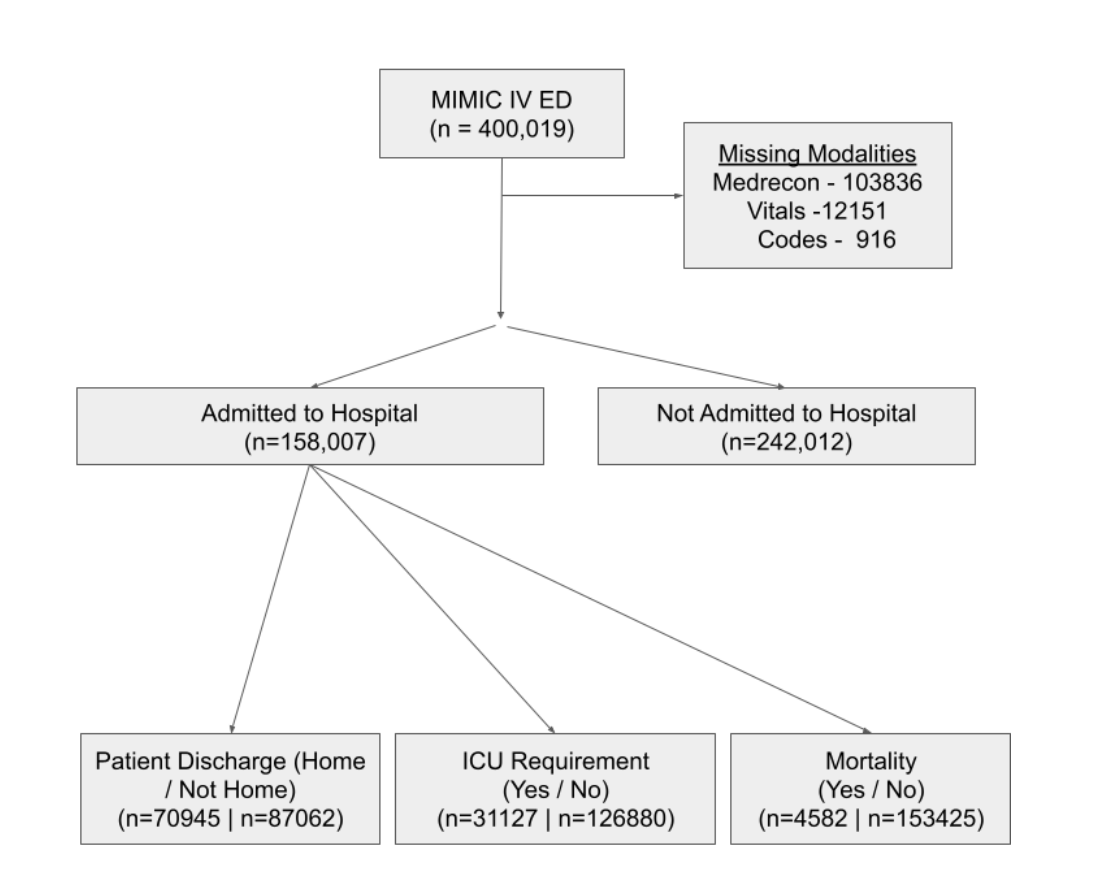
\includegraphics[width=4in]{strobe1.png} 
   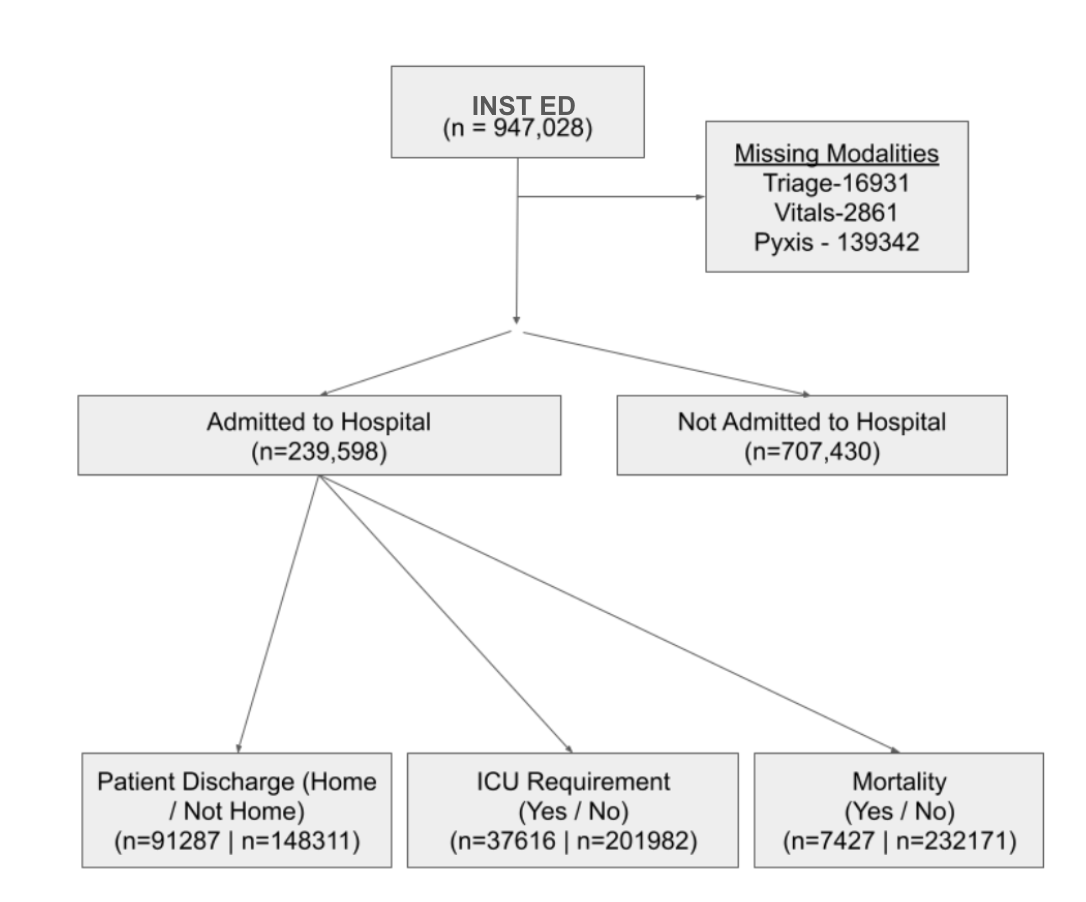
\includegraphics[width=4in]{strobe2.png} 
   \caption{Strobe Diagrams for both MIMIC-IV ED and our Institutional ED Dataset}
   \label{strobe} 
 \end{figure} 

\subsection{Example Pseudo-notes}
\label{exnotes}
\begin{multicols}{2}

\noindent\textit{Arrival Information}\\
\fbox{\begin{minipage}{18em}
The Patient is a {52} year old {white female}, arrived via {ambulance} at {2180-05-06 19:17:00}. The patient's marital status is {widowed}. The patient's insurance is {other}. The patient's language is {english}.
\end{minipage}}

\noindent\textit{Emergency Department Disposition}\\
\fbox{\begin{minipage}{18em}
The ED disposition was {admitted} at {2180-05-06 23:30:00}. The patient died on {2180-09-09}.
\end{minipage}}

\noindent\textit{Diagnostic Codes}\\
\fbox{\begin{minipage}{18em}
The patient received the following diagnostic codes: ICD-9 code: {[78959], other ascites}. ICD-9 code: {[07070], unspecified viral hepatitis c without hepatic coma}. ICD-9 code: {[5715], cirrhosis of liver nos}. ICD-9 code: {[v08], asymptomatic hiv infection}. 
\end{minipage}}

\noindent\textit{Medrecon}\\ 
\fbox{\begin{minipage}{18em}
The patient was previously taking the following medications: {albuterol sulfate}, {asthma/copd therapy - beta 2-adrenergic agents}, {inhaled}, {short acting}. {peg 3350-electrolytes}, {laxative - saline/osmotic mixtures}. {nicotine}, {smoking deterrents - nicotine-type}. {spironolactone [aldactone]}, {aldosterone receptor antagonists}. {emtricitabine-tenofovir [truvada]}, {antiretroviral - nucleoside and nucleotide analog rtis combinations}. {raltegravir [isentress]}, {antiretroviral - hiv-1 integrase strand transfer inhibitors}. {spironolactone [aldactone]}, {diuretic - aldosterone receptor antagonist}, {non-selective}. {furosemide, diuretic - loop}. {ipratropium bromide [atrovent hfa]}, {asthma/copd - anticholinergic agents}, {inhaled short acting}. {ergocalciferol (vitamin d2)}, {vitamins - d derivatives}.
\end{minipage}} 

\noindent\textit{Patient Vitals}\\
\fbox{\begin{minipage}{18em}
The patient had the following vitals: At {2180-05-06 23:04:00}, temperature was {97.7}, pulse was {79}, respirations was {16}, o2 saturation was {98}, systolic blood pressure was {107}, diastolic blood pressure was {60}, pain was {0}.
\end{minipage}} 

\noindent\textit{Pyxis}\\
\fbox{\begin{minipage}{18em}
The patient received the following medications: At {2180-08-05 22:29:00}, {morphine} were administered. At {2180-08-05 22:55:00}, {donnatol (elixir), aluminum-magnesium hydrox.-simet, aluminum-magnesium hydrox.-simet, ondansetron, ondansetron} were administered. 
\end{minipage}}

\noindent\textit{Triage}\\
\fbox{\begin{minipage}{18em}
At triage: temperature was {98.4}, pulse was {70}, respirations was {16}, o2 saturation was {97}, systolic blood pressure was {106}, diastolic blood pressure was {63}, pain was {0}, chief complaint was {abd pain}, {abdominal distention}. Acuity score was {3}.
\end{minipage}}

\end{multicols}

\subsection{Foundation Model Descriptions for Model Selection Experiment}
\label{model_des}

A Table of the foundation models that we used to select the MEME model along with their descriptions are found in Table \ref{TableModel}.

\begin{table}[H]
\caption{The foundation models evaluated for becoming the backbone for MEME.}
\begin{tabular}{p{6cm}p{8cm}}
\toprule
\textbf{Model} & \textbf{Description} \\
\midrule
\textbf{BioBERT} \citep{lee2020biobert} & A BERT variant pretrained on large biomedical corpora, enabling it to better capture domain-specific linguistic patterns and outperform general BERT on biomedical text mining tasks like named entity recognition, relation extraction, and question answering.\\
\midrule
\textbf{Bio\_ClinicalBERT} \citep{alsentzer2019publicly} & Initialized with BioBERT and further pretrained on clinical notes from the MIMIC III database (~880M words), this model is designed for tasks involving electronic health records from ICU patients.\\
\midrule
\textbf{ClinicalBERT} \citep{huang2019clinicalbert} & Pretrained on a large clinical corpus of 1.2B words spanning diverse diseases and fine-tuned on over 3 million electronic health records, this model is well-suited for clinical NLP tasks due to its understanding of medical terminology and health record data.\\
\midrule
\textbf{DistilBERT} \citep{sanh2019distilbert} & A lightweight and faster version of BERT, designed for efficient inference on resource-constrained devices while retaining most of BERT's performance on various NLP tasks.\\
\midrule
\textbf{MedBERT} \citep{9980157} & A model initialized with Bio\_ClinicalBERT and further pretrained on biomedical datasets like N2C2, BioNLP, and CRAFT, tailored for biomedical named entity recognition tasks involving diseases, drugs, genes, and other healthcare concepts.\\
\midrule
\textbf{T5} \citep{2020t5} & Pretrained on a massive text corpus using a text-to-text denoising objective, this encoder-decoder transformer model can be flexibly applied to various NLP tasks like translation, summarization, and question answering by framing them as text-to-text problems.\\
\midrule
\textbf{XLNet} \citep{yang2019xlnet} & A generalized autoregressive pretraining method that combines the advantages of autoregressive language modeling and the permutation-based approaches used in BERT. It captures bidirectional contexts by maximizing the expected likelihood over all permutations of the input sequence factorization order.\\
\bottomrule
\label{TableModel}
\end{tabular}
\end{table}

% \subsection{Model Descriptions}
% In the subsequent section, we get ino into the \iffalse intricate \fi details of the model architectures employed by other single modality approaches and \iffalse proficient \fi machine learning methods. \iffalse , offering a comprehensive exploration for pedagogical clarity. \fi We disclose more detailed hyperparameters and architectural designs that constitute these models, facilitating a transparent benchmarking process. If there are any further questions after reading this section, feel free to contact the authors for more details. \\

% \noindent\textbf{Single Modality Specific  Methods}\\
% In our analysis, we presented six distinct model variations, each tailored to one of the six modalities used for predicting the target variable. While these models share similarities with our multimodal approach, they diverge in certain aspects as deliberate feature removal sets them apart from our multimodal methodology. These single modality approaches adhere to a more conventional Language Model (LLM) fine-tuning paradigm. However they still do slightly diverge from these approaches as well. In these single modality models, we froze each LLM encoder and trained a linear classifier to be able to learn the proper underlying representations to make a proper prediction.

% Moreover, unlike our multimodal model, these single modality models forego our second step to the network, which incorporates an additional self-attention layer step, as they do not necessitate learning a unified input. This \iffalse streamlined \fi approach reflects the task-specific focus of these models, optimizing for individual modality predictions without the need for a unified multimodal analysis.

% In terms of preprocessing, we used the same preprocessing steps as our multimodal approach and extracted the modality-specific subset Dataset object from the Hugging Face library for our analysis. Subsequently, we loaded these dataset objects into conventional PyTorch dataloaders for training the classifier. Similar to our multimodal approach, we also utilized the Cross-Entropy Loss and AdamW optimizer, with a learning rate of $5e-5$, and trained until the validation error converges. Additionally, we implemented a linear learning rate scheduler to adjust the model’s learning rate during training, thus tuning this hyperparameter, which impacts our overall model performance. We tracked F1 scores to assess the performance of our model after every epoch. \\ 

% \noindent\textbf{Multimodal Single Embedding Model}\\
% In our benchmarking study, we also included a model referred to as the Multimodal Single Embedding Model (MSEM). This inclusion represents the canonical LLM approach of \iffalse aimed to preemptively address potential queries about \fi consolidating all text data into a single embedding. The MSEM closely resembles single modality models in terms of architecture; however, it diverges primarily in its preprocessing step, where all text is merged into a single column and truncated during tokenization.

% The feasibility of an MSEM is largely constrained by context-length limitations imposed by BERT and other Large Language Models (LLMs). In our study, we focused on Emergency department EHR data, which encompassed six corresponding modalities. However, in broader applications like general EHR, the data can span as many as 10-20 different modalities related to a patient's health history. These limitations are significant as they potentially restrict the depth and breadth of data that can be effectively processed and analyzed by models like the MSEM. \\

% \noindent\textbf{Random Forest Classifier}\\
% Lastly, our benchmarking also involved training and fitting a Random Forest classifier. \iffalse Renowned as an ensemble learning technique, Random Forest is part of the decision tree-based algorithm family. Its strength lies in constructing multiple decision trees whose collective outputs are aggregated to yield predictions that are both robust and accurate. \fi We selected 1000 estimators, equivalent to creating 1000 trees. \iffalse Given our ample resources, handling this substantial number of estimators was feasible, thus influencing our choice of this particular hyperparameter. \fi 
% In contrast to our approach with pseudo-notes, the data preparation for the Random Forest classifier was markedly different. While BERT and transformer-based models primarily process text data, such an approach was not viable with the Random Forest. Consequently, we utilized the EHR data in its unaltered tabular format. To maintain consistency across our analyses, we filtered this data using the same patient subsets identified in the test, validation, and training sets of our transformer-based methods. Furthermore, we implemented one-hot encoding on various modalities, including medication reconciliation, ICD codes, and Pyxis drugs, to effectively prepare the data for the Random Forest model.


\subsection{Ablation Study Table}
\label{ablation}

We display the raw performance metrics from our ablation study of the various modalities contributing to the multiple tasks proposed in our work on the MIMIC IV ED dataset. The complete set of results is displayed in Tables \ref{r4}, \ref{r5}, \ref{r6}}. We note that no modality alone beat out the MEME model which took on a multimodal approach. 

\begin{table}[H]
\caption{F1 Scores for MIMIC-IV ED Dataset Ablation Study Across Different Tasks.}
\label{r4}
\begin{adjustbox}{width=\textwidth}
\begin{small}
\begin{sc}
\begin{tabular}{l|c|ccc}
\toprule
F1 Benchmark & Dispositon & & Decompensation &\\
Modality & ED Disposition & Discharge & ICU & Mortality \\
\midrule
Arrival & 0.895 $\pm$ 0.003 & 0.533 $\pm$ 0.008 & 0.041 $\pm$ 0.009 & 0.063 $\pm$ 0.005 \\
Codes & 0.613 $\pm$ 0.003 & 0.572 $\pm$ 0.008 & 0.054 $\pm$ 0.009 & 0.055 $\pm$ 0.004 \\
Medrecon & 0.625 $\pm$ 0.005 & 0.525 $\pm$ 0.009 & 0.029 $\pm$ 0.005 & 0.054 $\pm$ 0.004 \\
Pyxis & 0.564 $\pm$ 0.004 & 0.478 $\pm$ 0.009 & 0.167 $\pm$ 0.015 & 0.060 $\pm$ 0.005 \\
Triage & 0.596 $\pm$ 0.005 & 0.403 $\pm$ 0.010 & 0.367 $\pm$ 0.015 & 0.055 $\pm$ 0.004 \\
Vitals & 0.619 $\pm$ 0.005 & 0.366 $\pm$ 0.009 & 0.160 $\pm$ 0.013 & 0.067 $\pm$ 0.006 \\
MEME & \textbf{0.943 $\pm$ 0.003} & \textbf{0.698 $\pm$ 0.007} & \textbf{0.572 $\pm$ 0.014} & \textbf{0.137 $\pm$ 0.035} \\
\bottomrule
\end{tabular}
\end{sc}
\end{small}
\end{adjustbox}
\end{table}

\begin{table}[H]
\caption{AUROC Scores for MIMIC-IV ED Dataset Ablation Study Across Different Tasks.
}
\label{r5}
\begin{adjustbox}{width=\textwidth}
\begin{small}
\begin{tabular}{l|c|ccc}
\toprule
AUROC Benchmark & Dispositon & & Decompensation &\\
Modality & ED Disposition & Discharge & ICU & Mortality \\
\midrule
Arrival & 0.940 $\pm$ 0.002 & 0.689 $\pm$ 0.007 & 0.682 $\pm$ 0.009 & 0.709 $\pm$ 0.019 \\
Codes & 0.715 $\pm$ 0.005 & 0.658 $\pm$ 0.007 & 0.714 $\pm$ 0.008 & 0.709 $\pm$ 0.020 \\
Medrecon & 0.709 $\pm$ 0.004 & 0.644 $\pm$ 0.007 & 0.622 $\pm$ 0.009 & 0.668 $\pm$ 0.021 \\
Pyxis & 0.498 $\pm$ 0.005 & 0.616 $\pm$ 0.008 & 0.704 $\pm$ 0.009 & 0.705 $\pm$ 0.024 \\
Triage & 0.677 $\pm$ 0.004 & 0.647 $\pm$ 0.007 & 0.758 $\pm$ 0.008 & 0.736 $\pm$ 0.020 \\
Vitals & 0.720 $\pm$ 0.004 & 0.598 $\pm$ 0.008 & 0.733 $\pm$ 0.008 & 0.740 $\pm$ 0.021 \\
MEME & \textbf{0.991 $\pm$ 0.001} & 0.\textbf{799 $\pm$ 0.006} & \textbf{0.870 $\pm$ 0.015} & \textbf{0.862 $\pm$ 0.006} \\
\bottomrule
\end{tabular}
\end{small}
\end{adjustbox}
\end{table}

\begin{table}[H]
\caption{AUPRC Scores for MIMIC-IV ED Dataset Ablation Study Across Different Tasks.}
\label{r6}
\begin{adjustbox}{width=\textwidth}
\begin{small}
\begin{tabular}{l|c|ccc}
\toprule
AUPRC Benchmark & Dispositon & & Decompensation &\\
Model & ED Disposition & Discharge & ICU & Mortality \\
\midrule
Arrival & 0.861 $\pm$ 0.005 & 0.625 $\pm$ 0.010 & 0.376 $\pm$ 0.014 & 0.076 $\pm$ 0.013 \\
Codes & 0.645 $\pm$ 0.007 & 0.595 $\pm$ 0.011 & 0.410 $\pm$ 0.014 & 0.061 $\pm$ 0.008 \\
Medrecon & 0.589 $\pm$ 0.007 & 0.579 $\pm$ 0.010 & 0.286 $\pm$ 0.010 & 0.049 $\pm$ 0.006 \\
Pyxis & 0.391 $\pm$ 0.005 & 0.561 $\pm$ 0.011 & 0.484 $\pm$ 0.015 & 0.112 $\pm$ 0.022 \\
Triage & 0.552 $\pm$ 0.008 & 0.579 $\pm$ 0.011 & 0.504 $\pm$ 0.015 & 0.100 $\pm$ 0.017 \\
Vitals & 0.623 $\pm$ 0.007 & 0.544 $\pm$ 0.010 & 0.430 $\pm$ 0.014 & 0.087 $\pm$ 0.014 \\
MEME & \textbf{0.983 $\pm$ 0.002} & \textbf{0.765 $\pm$ 0.008} & \textbf{0.709 $\pm$ 0.012} & \textbf{0.243 $\pm$ 0.034} \\

\bottomrule
\end{tabular}
\end{small}
\end{adjustbox}
\end{table}
\newpage
\subsection{GPT3.5-Turbo Prompt}

\begin{lstlisting}[language=Python, caption=Basic Example of How prompted the gpt-3.5-turbo model to generate predictions.]
from openai import OpenAI
client = OpenAI()

completion = client.chat.completions.create(
  model="gpt-3.5-turbo",
  messages=[
    {"role": "system", "content": "You are a medical officer, skilled in determining whether a patient should be admitted to the Emergency Room or not."},
    {"role": "user", "content": "I have 10 patient samples here. I need you to predict whether each patient should be admitted to the emergency room or not. Give you prediction in the list format ([`1,0,0,1,1,1,0,1,0,1']) and predict 1 if they should be admitted and 0 if not:\n\n'Patient 10000032, a 52 year old white female, arrived via ambulance at 2180-05-06 19:17:00. The patient's marital status is widowed. The patient's insurance is other. The patient's language is english.The patient received the following diagnostic codes: ICD-9 code: [5728], oth sequela, chr liv dis. ICD-9 code: [78959], other ascites. ICD-9 code: [07070], unspecified viral hepatitis c without hepatic coma. ICD-9 code: [v08]...'

    ...
    [OTHER_PSEUDONOTES]
    ...
    "}
  ]
)

print(completion.choices[0].message)

>>> Here are the predictions: {"predictions": [1, 0, 1, 1, 1, 1, 1, 1, 1, 1]}
\end{lstlisting}

\subsection{Why did Generalization Fail?}
\label{gener3}

% \begin{figure}[h!] 
%     \centering
%     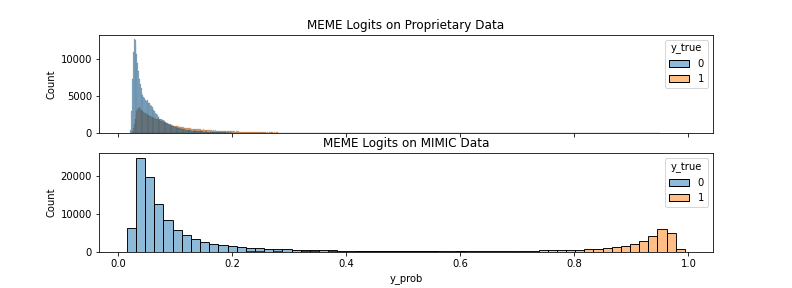
\includegraphics[width=\textwidth]{logits.png}
%     \caption{The Logits Generated from Running MEME on MIMIC IV versus Institutional Dataset}
%     \label{fig:enter-label}
% \end{figure}

To investigate the failure of our generalization experiment from MIMIC to our institutional database, we conducted a thorough examination of the data input into our pseudo-notes method. We analyzed the data from both Electronic Health Record (EHR) sources by plotting distributions via box plots, and Venn diagrams to elucidate the disparities between the datasets.

\subsubsection*{Arrival Information}

All results related to \textit{arrival} information are presented in Figure \ref{app1}. We observe notable differences within these extensive categorical classes for arrival transport and race labels. Although these differences are not considered substantial, highlighting these disparities remains critical.

\begin{figure}[h!]
   \centering 
   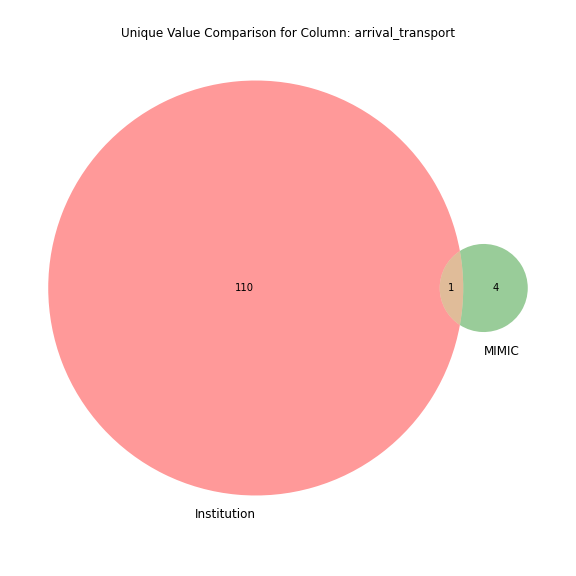
\includegraphics[width=4.5in]{plots/arrival_transport_venn.png} 
   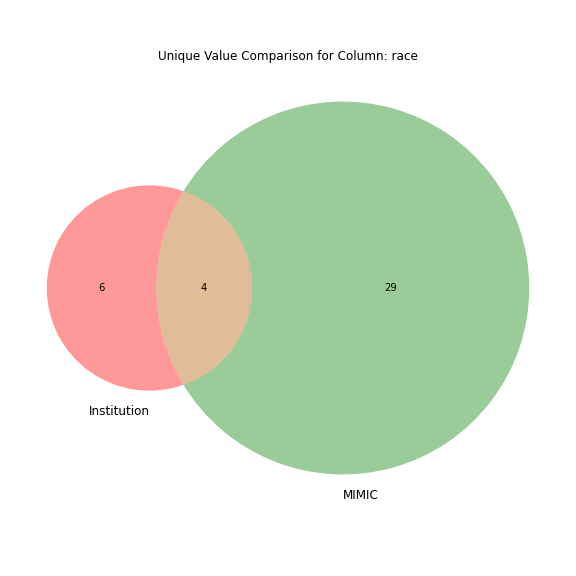
\includegraphics[width=4.5in]{plots/race_venn.png} 
   \caption{The Venn diagram illustrates the overlap between unique elements identified in our Institutional Data and MIMIC-IV ED \textbf{Arrival} Information Data.}
   \label{app1} 
 \end{figure} 

 \subsubsection*{Diagnoses}
All results pertaining to \textit{diagnoses }information are presented in Figure \ref{app2}. We observe notable differences within the ICD Diagnostic codes. These differences are critical and may contribute to failed generalization.
 
 \begin{figure}[h!]
   \centering 
   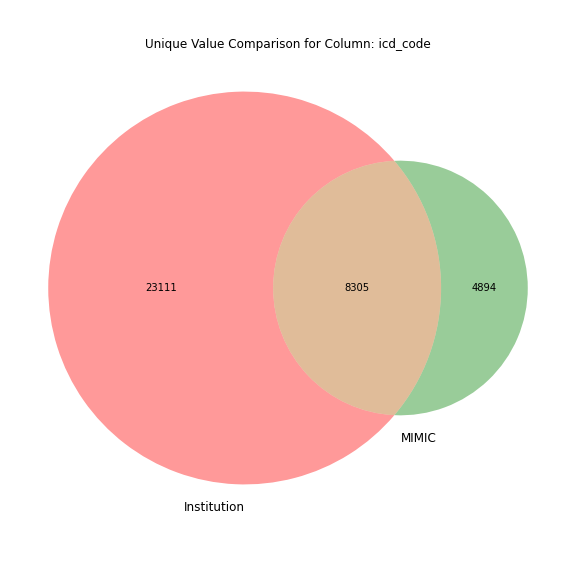
\includegraphics[width=4.5in]{plots/icd_code_venn.png} 
   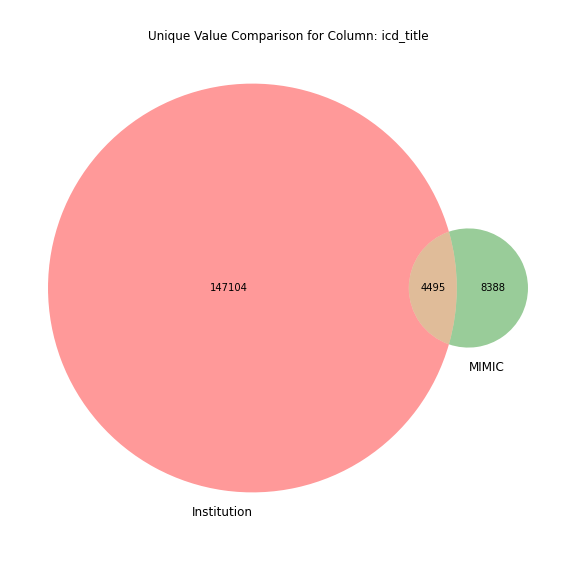
\includegraphics[width=4.5in]{plots/icd_title_venn.png} 
   \caption{The Venn diagram illustrates the overlap between unique elements identified in our Institutional Data and MIMIC-IV ED \textbf{Diagnoses} Data.}
   \label{app2} 
 \end{figure} 

 \subsubsection*{Pyxis}
 All results pertaining to \textit{pyxis} information are presented in Figure \ref{app3}. We observe notable differences within the drug names dispensed during their ED Visit. These differences are critical and may contribute to failed generalization.
 \begin{figure}[h!]
   \centering 
   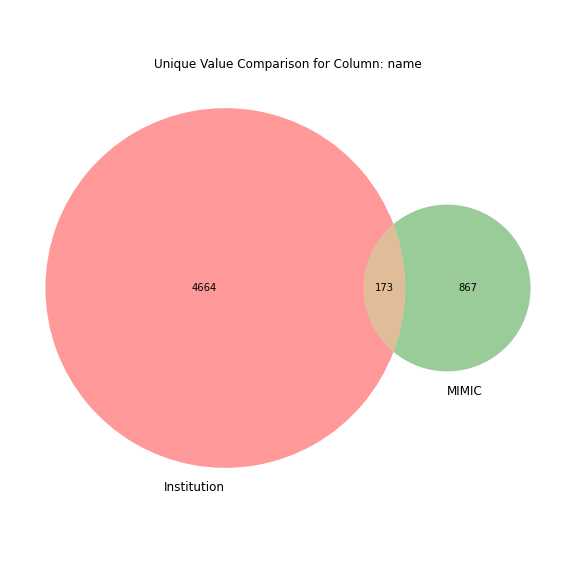
\includegraphics[width=5in]{plots/name_venn.png} 
   \caption{The Venn diagram illustrates the overlap between unique elements identified in our Institutional Data and MIMIC-IV ED \textbf{Pyxis} Data.}
   \label{app3} 
 \end{figure} 

 \subsubsection*{Triage}
All results related to \textit{pyxis} information are presented in Figures \ref{app4} and \ref{app5}. We observe notable differences in the chief complaints, which were anticipated to vary. However, we emphasize that numerical values within EHRs appeared as expected and exhibited similar distributions with marginal outliers. These differences are critical and may contribute to failed generalization.

\begin{figure}[h!]
   \centering 
   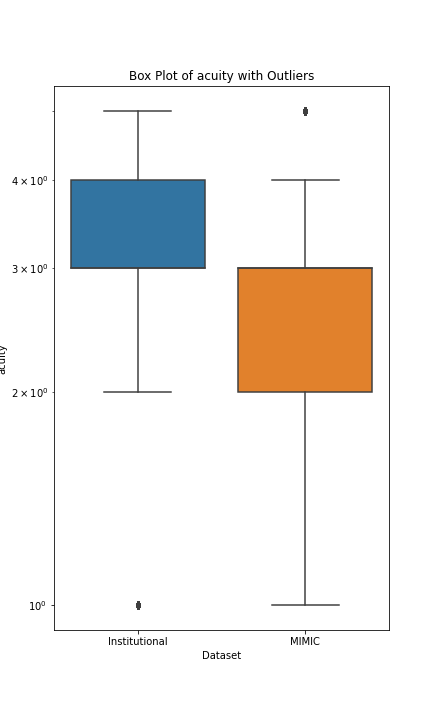
\includegraphics[width=2.5in]{plots/acuity_triage_boxplot.png} 
   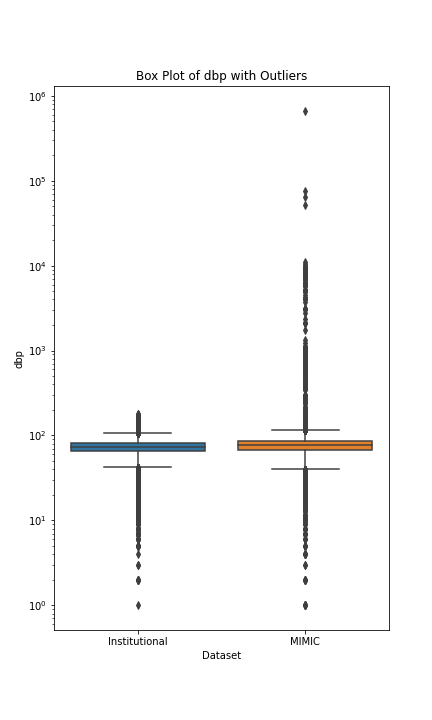
\includegraphics[width=2.5in]{plots/dbp_triage_boxplot.png} 
   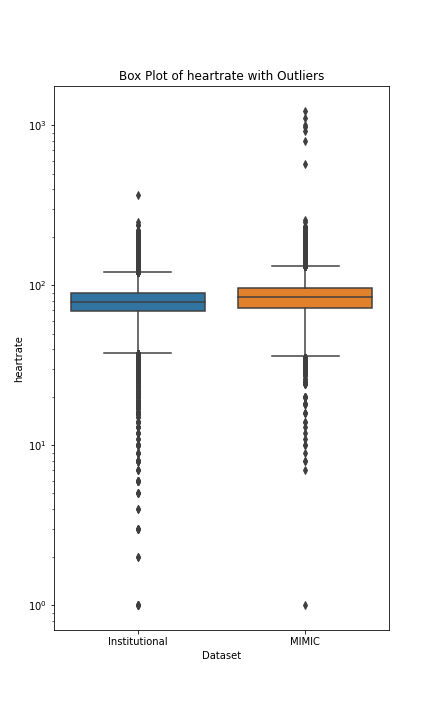
\includegraphics[width=2.5in]{plots/heartrate_triage_boxplot.png} 
   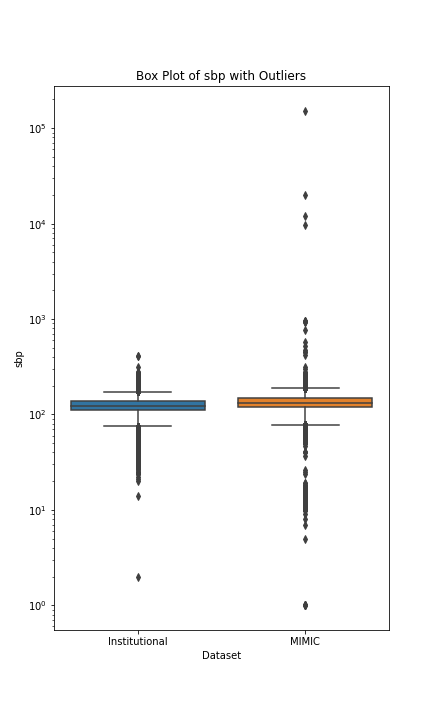
\includegraphics[width=2.5in]{plots/sbp_triage_boxplot.png} 
   \caption{The box plot depicts the distribution of values within Institutional and MIMIC-IV ED \textbf{Triage Information} Datasets, thereby facilitating a comparative analysis of data variability and central tendency across the datasets.}
   \label{app4} 
 \end{figure} 

 \begin{figure}[h!]
   \centering 
   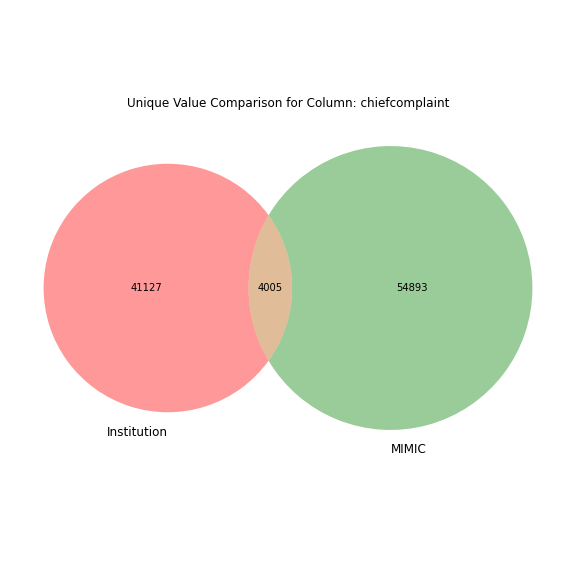
\includegraphics[width=5in]{plots/chiefcomplaint_venn.png} 
   \caption{The Venn diagram illustrates the overlap between unique elements identified in our Institutional Data and MIMIC-IV ED \textbf{Chief Complaints} Data coming from \textbf{Triage} Information.}
   \label{app5} 
 \end{figure} 

 \subsubsection*{Vitals}
All results related to \textit{vitals} information are presented in Figures \ref{app6}. We see again that numerical data appears to follow similar distributions despite a few outliers. We do not think the numerical aspects of the EHR led to failed generalization.
\begin{figure}[h!]
   \centering 
   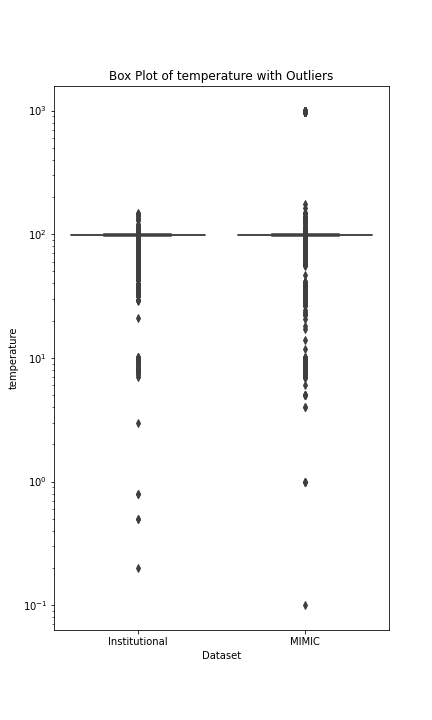
\includegraphics[width=2.5in]{plots/temperature_boxplot.png} 
   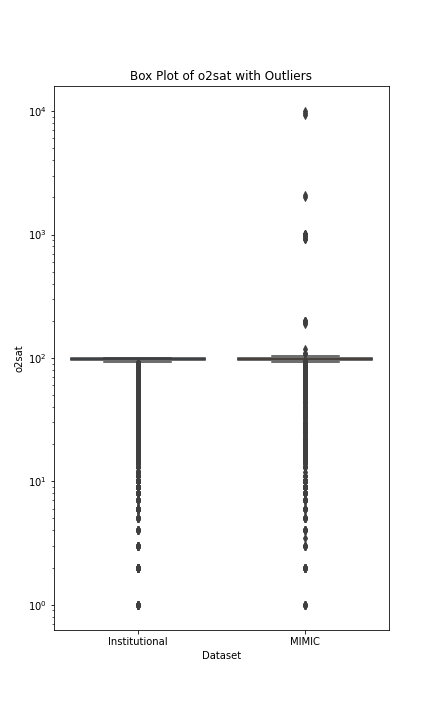
\includegraphics[width=2.5in]{plots/o2sat_boxplot.png} 
   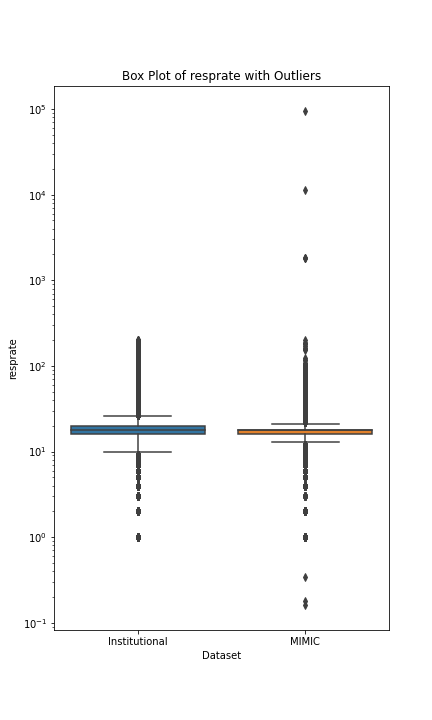
\includegraphics[width=2.5in]{plots/resprate_boxplot.png} 
   \caption{The box plot depicts the distribution of values within Institutional and MIMIC-IV ED \textbf{Vitals Information} Datasets, thereby facilitating a comparative analysis of data variability and central tendency across the datasets.}
   \label{app6} 
 \end{figure} 

\subsection*{Remarks based on Analysis}

Our analysis reveals that EHR systems exhibit significant variability especially in the case of free text and categorical data types. This diversity is evident in the unique chief complaints, diagnostic annotations, and other unique medical cases of different hospital institutions, which contribute to the challenges in achieving generalization. These insights underscore the complexities inherent in working across heterogeneous EHR environments and advise to use this method with some local fine-tuning of hospitals as highlighted in \citep{jiang2023health}.

\end{document}
